% % % % % % % % % % % % % % % % % % % % % % % % % % % % % % % % % % % % % % % % % % % %
%                                                                                     %
% Short Sectioned Assignment LaTeX Template Version 1.0 (5/5/12)                      %
% This template has been downloaded from: http://www.LaTeXTemplates.com               %
%                                                                                     %
% Original author:  Frits Wenneker (http://www.howtotex.com)                          %
%                                                                                     %
% Modified by: Fco Javier Sueza Rodríguez (fcosueza@disroot.org)                      %
%                                                                                     %
% Changes:                                                                            %
%	    - Custom Chapters, Sections and Subsections (titlesec package)                %
%           - Document type scrbook (oneside)                                         %
%           - Use babel-lang-spanish package and marvosym                             %
%           - Use hyperref, enumitem, tcolorbox and glossaries packages               %
%           - Use Time New Roman (mathptmx), Helvetic and Courier fonts               %
%                                                                                     %
% License: CC BY-NC-SA 3.0 (http://creativecommons.org/licenses/by-nc-sa/3.0/)        %
%                                                                                     %
% % % % % % % % % % % % % % % % % % % % % % % % % % % % % % % % % % % % % % % % % % % %

%-----------------------------------------------%
%	              Packages                  %
%-----------------------------------------------%

\documentclass[paper=a4, fontsize=11pt, oneside]{scrbook}

% ---- Text Input/Output ----- %

\usepackage[T1]{fontenc}
\usepackage[utf8]{inputenc}
\usepackage{mathptmx}
\usepackage[scaled=.92]{helvet}
\usepackage{courier}
\usepackage[indent=12pt]{parskip}

\usepackage{geometry}
\geometry{verbose,tmargin=3cm,bmargin=3cm,lmargin=2.6cm,rmargin=2.6cm}

% ---- Language ----- %

\usepackage[spanish]{babel}
\usepackage{marvosym}

% ---- Another packages ---- %

\usepackage{amsmath,amsfonts,amsthm}
\usepackage{graphics,graphicx}
\usepackage{titlesec}
\usepackage{fancyhdr}
\usepackage{tcolorbox}
\usepackage{hyperref}
\usepackage{enumitem}
\usepackage[automake]{glossaries}

%--------------------------------------------------------------------%
%                      Customizing Document                          %
%--------------------------------------------------------------------%


% ----------- Custom Chapters, Sections and Subsections -------------- %

\titleformat{\chapter}[display]
			{\bfseries\Huge}
			{Tema \ \thechapter} {0.5ex}
			{\vspace{1ex}\centering}

\titleformat{\section}[hang]
			{\bfseries\Large}
			{\thesection}{0.5em}{}

\titleformat{\subsection}[hang]
			{\bfseries\large}
			{\thesubsection}{0.5em}{}

\titleformat{\subsubsection}[hang]
			{\bfseries\large}
			{\thesubsubsection}{0.5em}{}

\hypersetup{
    colorlinks=true,
    linkcolor=black,
    urlcolor=magenta
}

% ------------------- Custom heaaders and footers ------------------- %

\pagestyle{fancyplain}

\fancyhead[]{}
\fancyfoot[L]{}
\fancyfoot[C]{}
\fancyfoot[R]{\thepage}

\renewcommand{\headrulewidth}{0pt} % Remove header underlines
\renewcommand{\footrulewidth}{0pt} % Remove footer underlines

\setlength{\headheight}{13.6pt} % Customize the height of the header

% --------- Numbering equations, figures and tables ----------------- %

\numberwithin{equation}{section} % Number equations within sections
\numberwithin{figure}{section} % Number figures within sections
\numberwithin{table}{section} % Number tables within sections

% ------------------------ New Commands ----------------------------- %

\newcommand{\horrule}[1]{\rule{\linewidth}{#1}} % Create horizontal rule command


%----------------------------------------------------------------------------------------
%	TÍTULO Y DATOS DEL ALUMNO
%----------------------------------------------------------------------------------------

\title{
    \vspace{10ex}
    \normalfont \normalsize
    \huge \textbf{Tarea 4: Optimización y Documentación}
}
\author{Francisco Javier Sueza Rodríguez}
\date{\normalsize\today}

%----------------------------------------------------------------------------------------
%                                     DOCUMENTO
%----------------------------------------------------------------------------------------
\begin{document}

\maketitle

\thispagestyle{empty}

\vspace{75ex}

\begin{center}
    \begin{tabular}{l l}
        \textbf{Centro}: & IES Aguadulce \\
        \textbf{Ciclo Formativo}: & Desarrollo Aplicaciones Web (Distancia)\\
        \textbf{Asignatura}: & Entornos de Desarrollo\\
       \textbf{Tema}: & Tema 4 - Optimización y Documentación\\
    \end{tabular}
\end{center}

\newpage

\tableofcontents

\newpage

\listoffigures

\newpage

\section{Caso Práctico}
En  BK tras la fase de diseño están codificando los distintos programas y funcionalidades.

Dado que en dicha tarea están participando diversas personas han decidido utilizar distintas herramientas que les proporciona el entorno de desarrollo para lograr un código optimizado y documentado, además para poder realizar un seguimiento de las distintas etapas en las que se encuentran los códigos y facilitar el trabajo en equipo han decidido utilizar una herramientas de control de versiones.

\section{Actividades}

\subsection{Actividad 1: Utiliza la herramientas de refactorización de Netbeans}

\subsubsection{Enunciado}
En todos los apartados donde aparezca XXX tendrás que sustituirlo por tus datos personales Apellido1Apellido2Nombre.

\begin{enumerate}
    \item Cambia el nombre de la clase Vehiculo por VehiculoXXX2223. Dentro de la clase Main cambia el nombre de la variable miVehiculo por miVehiculoXXX2223
    \item Introduce el método operativaVehiculosXXX2223, que englobe las sentencias de la clase Main que operan con el objeto miVehiculoXXX2223.
    \item Encapsula todos los atributos de la clase VehiculoXXX2223.
    \item Añade el parámetro cantidad de tipo entero con un valor predeterminado de 50 al método operativaVehiculosXXX2223.
\end{enumerate}

\subsubsection{Solución}

\begin{enumerate}
    \item En primer lugar, hemos cambiado el nombre de la clase Vehiculo añadiendo la terminación \textbf{SuezaRguezFco2223}, usando la opción \textit{refactor} de netbeans. en las siguientes capturas podemos ver el cambio.

    \begin{figure}[H]
        \centering
        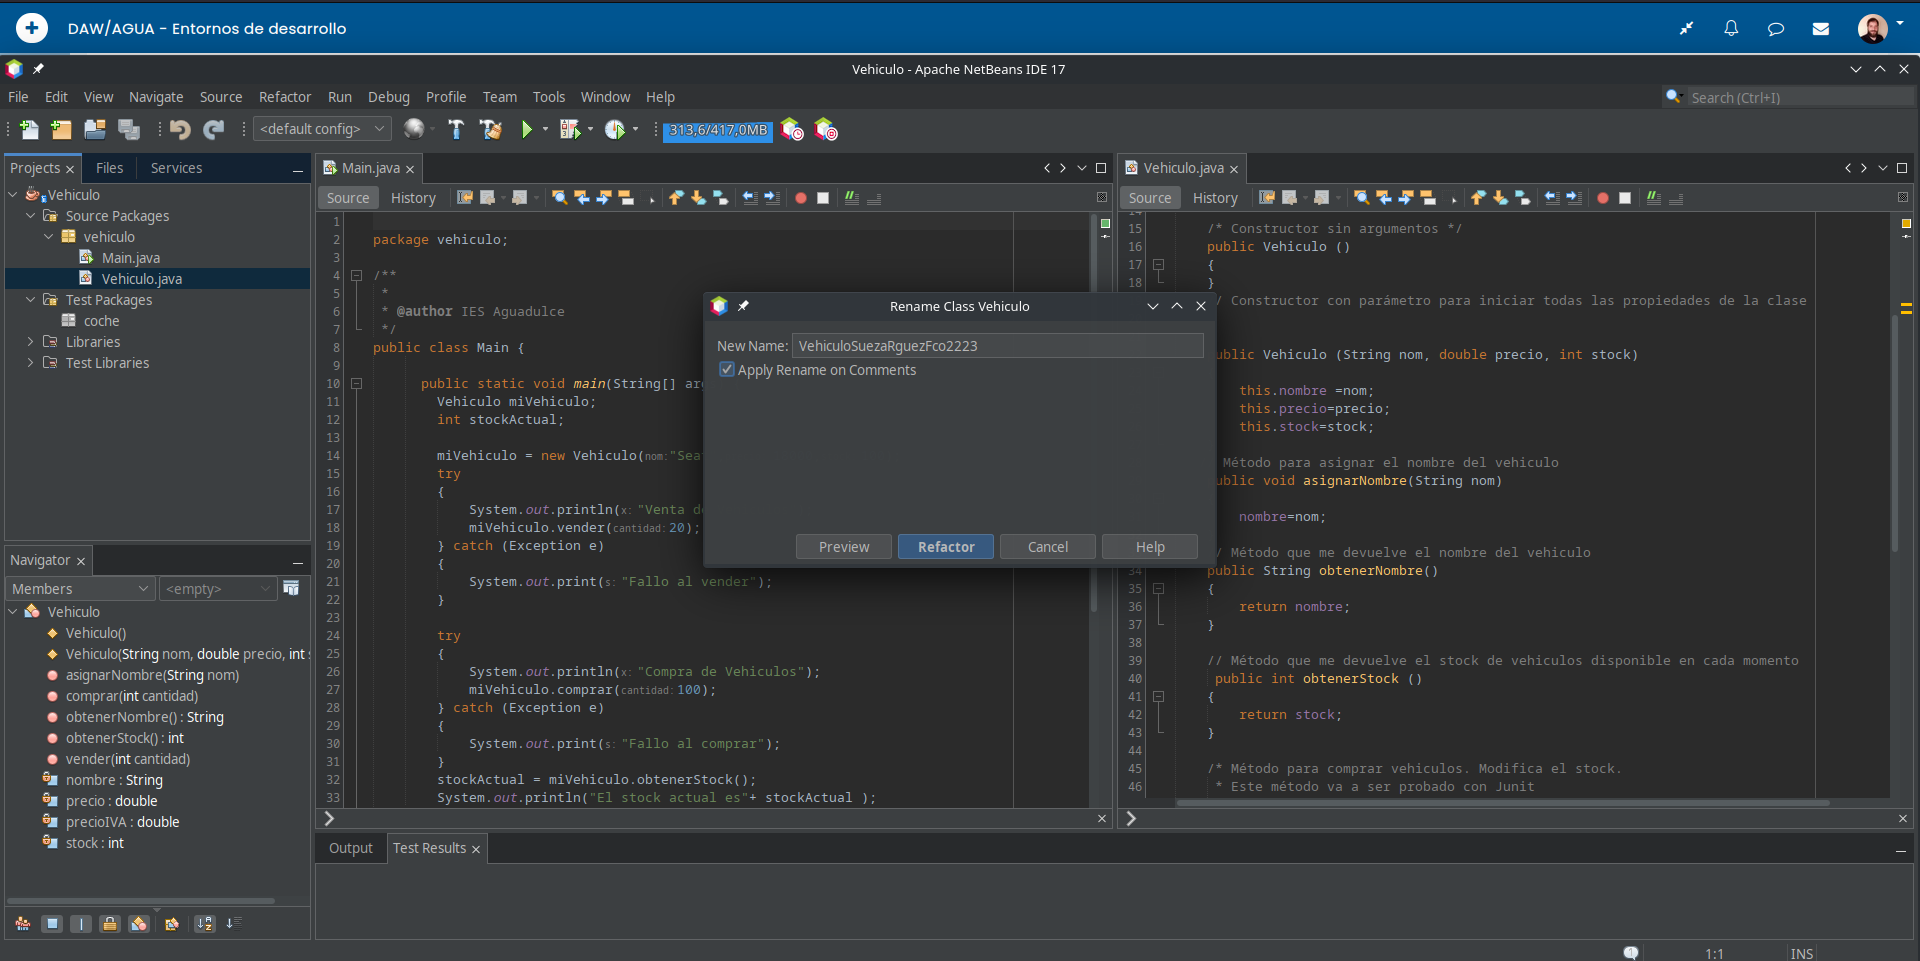
\includegraphics[scale=0.23]{refactor-class-1.png}
        \caption{Opción refactor de Netbeans}
    \end{figure}

    \begin{figure}[H]
        \centering
        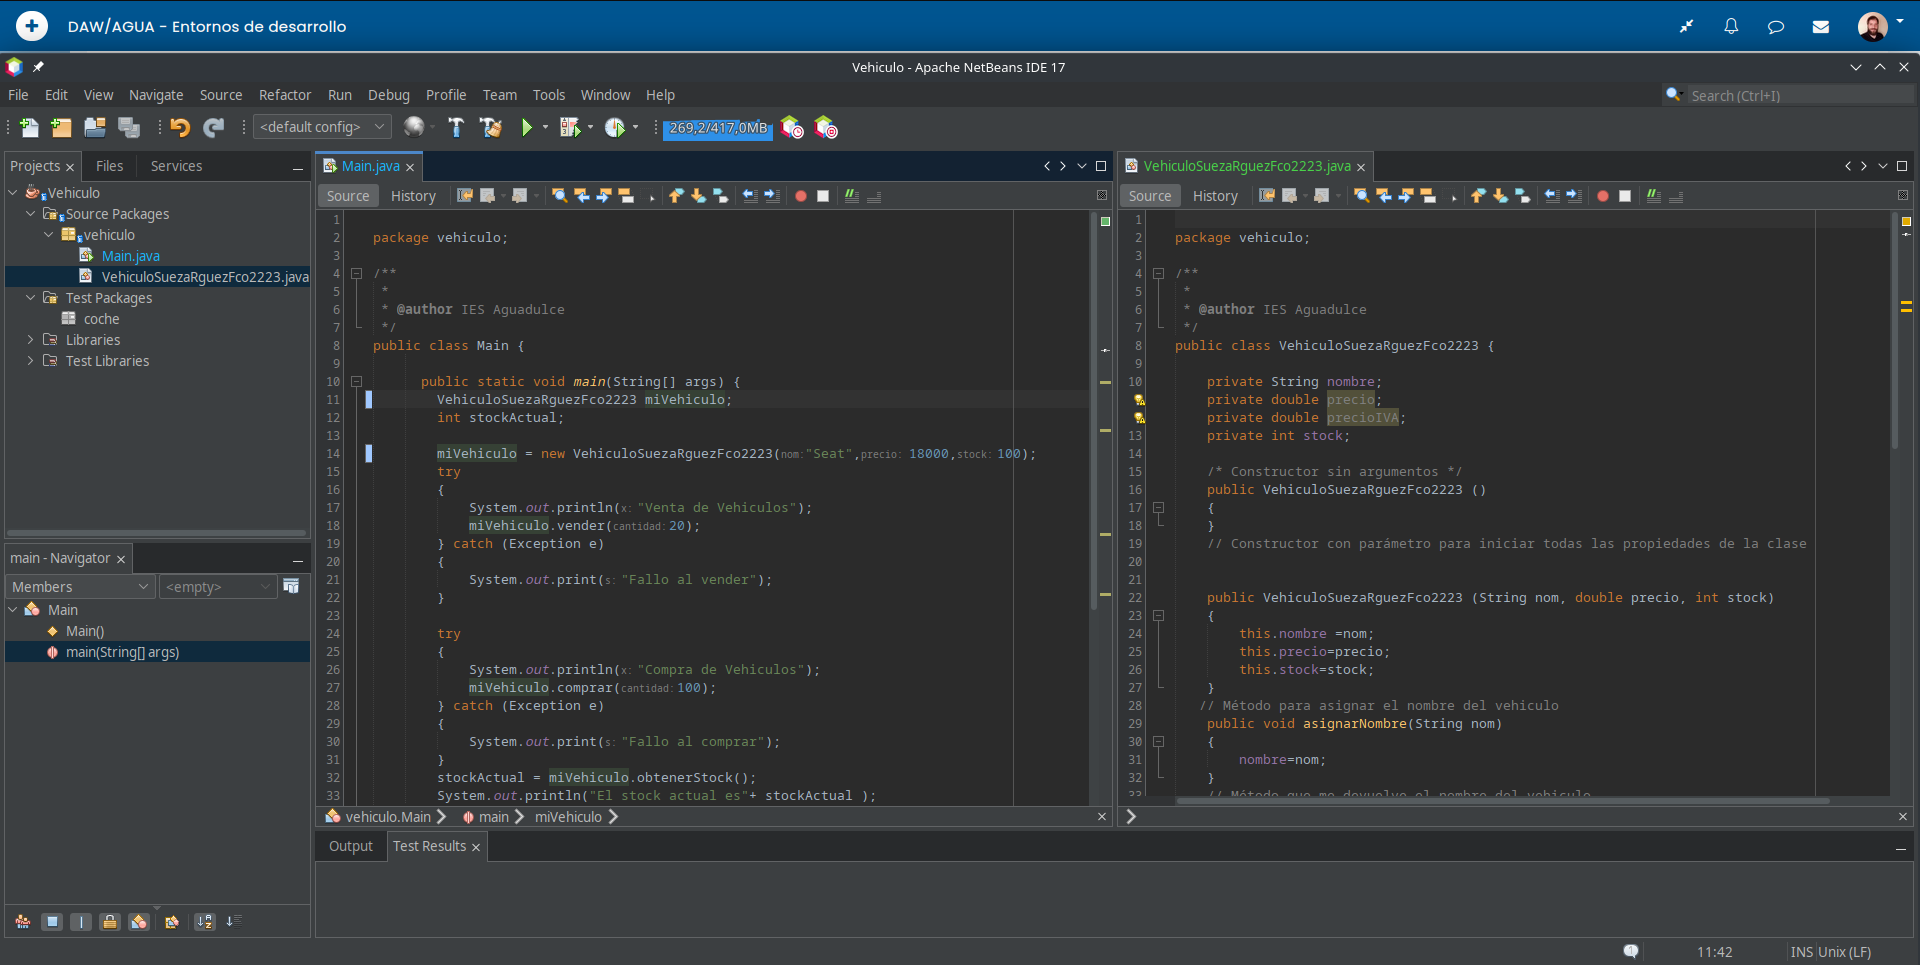
\includegraphics[scale=0.23]{refactor-class-2.png}
        \caption{Nombre de la clase Vehiculo cambiado}
    \end{figure}

    A continuación se ha cambiado el nombre de la variable miVehiculo en la clase Main, añadiendo la misma terminación.

    \begin{figure}[ht]
        \centering
        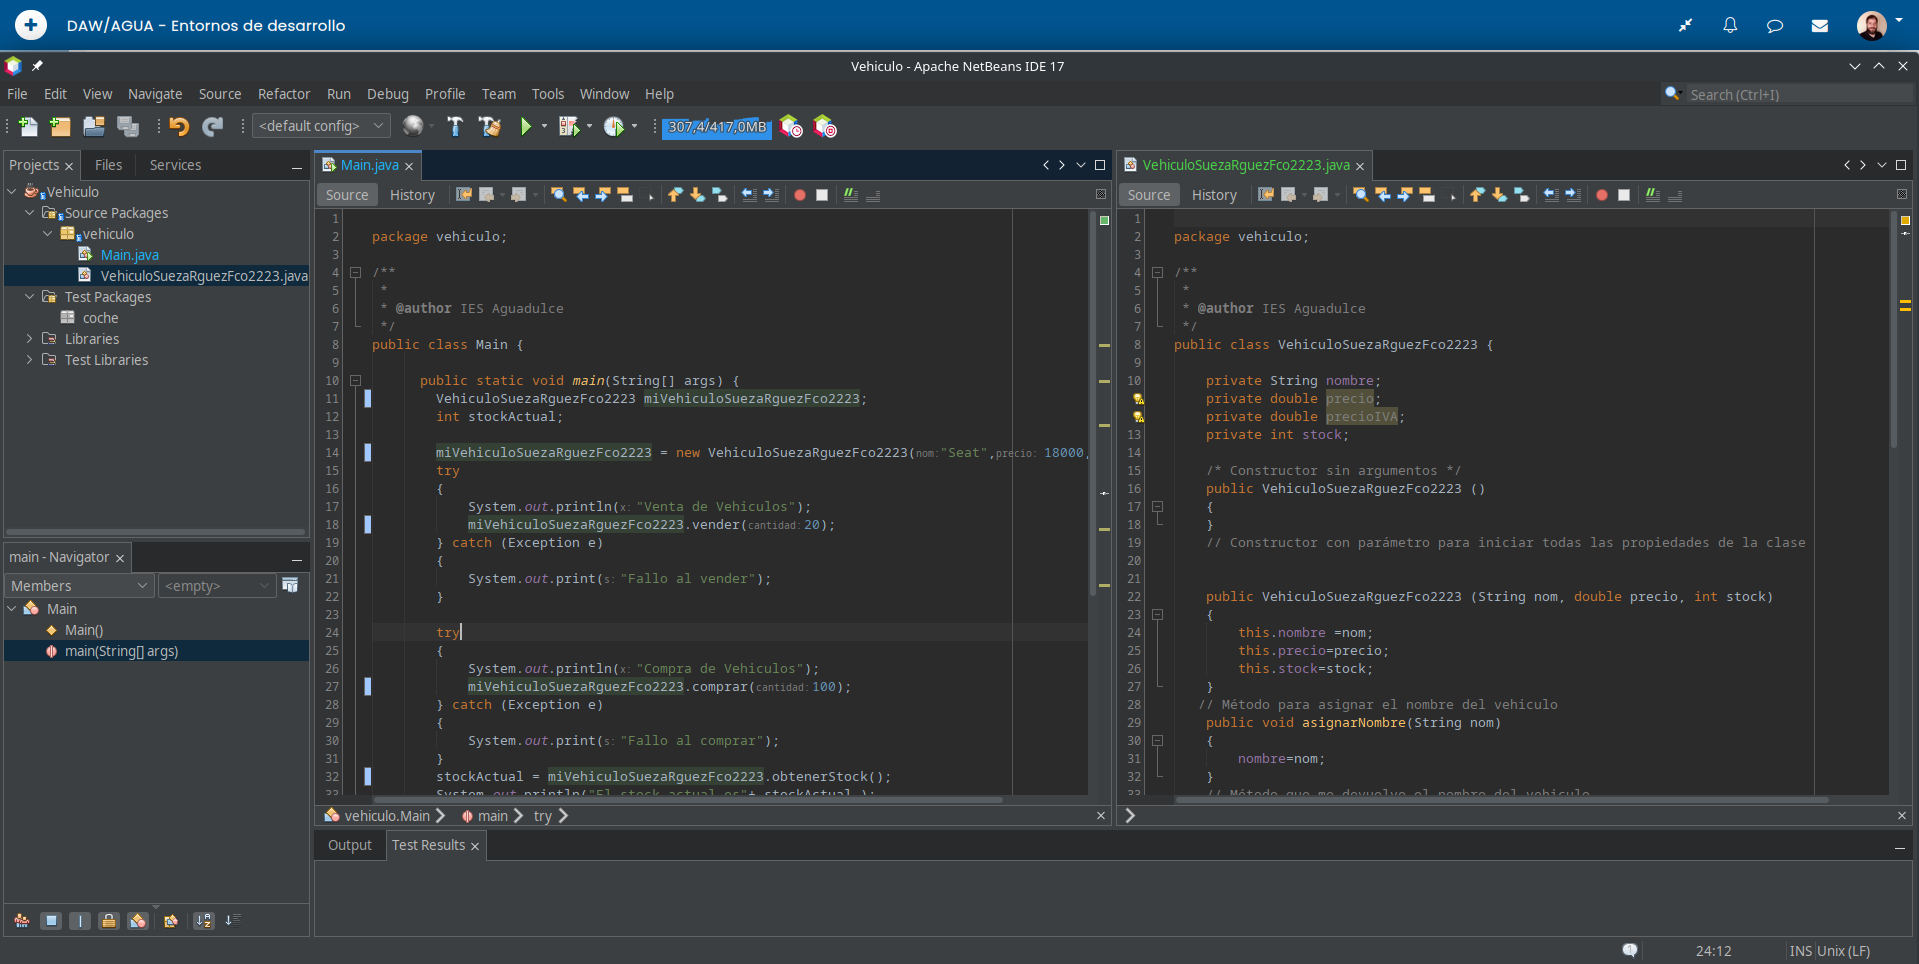
\includegraphics[scale=0.23]{refactor-var.png}
        \caption{Nombre de la variable miVehiculo cambiado}
    \end{figure}


    \item En este punto hemos refactorizado la clase Main e incluido todos los métodos que tratan con el objeto Vehiculo dentro de un método llamado operativaVehiculoSuezaRguezFco2223, usando para ello el menu refactor de Netbeans, con la opción \textit{introduce --> method}. En las siguiente capturas, se pueden ver los pasos seguidos.

    \begin{figure}[H]
        \centering
        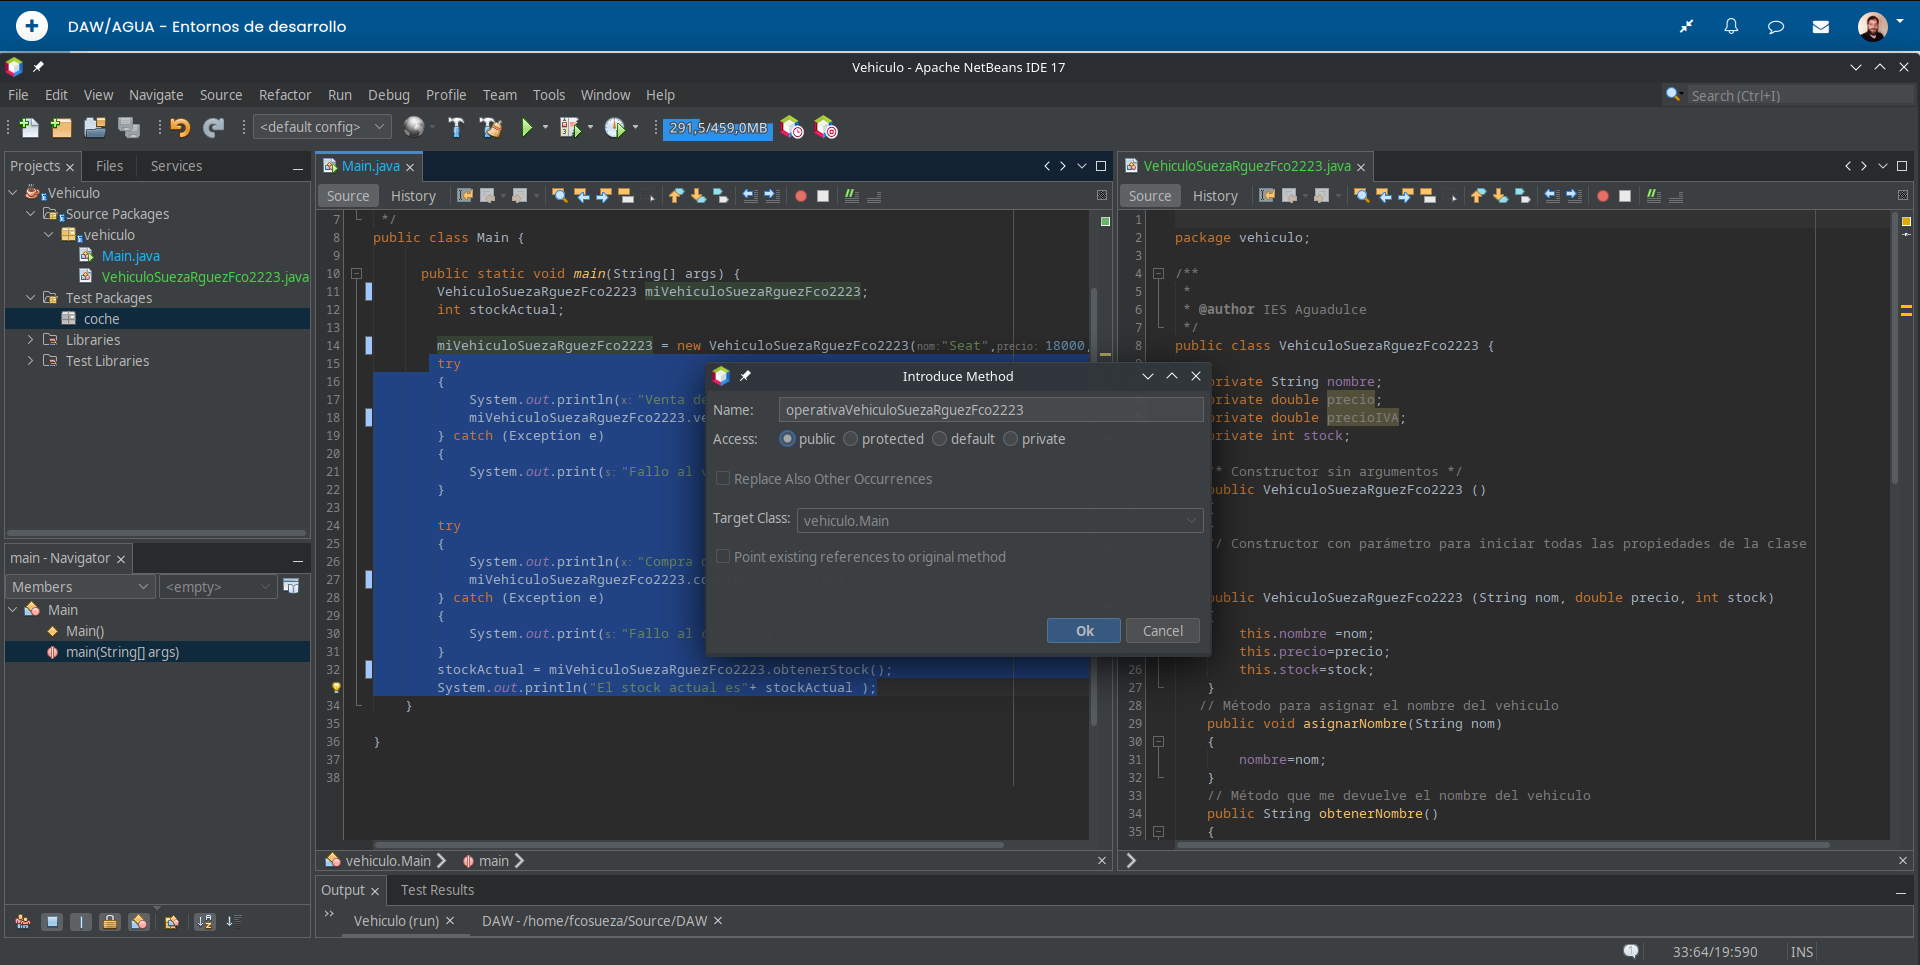
\includegraphics[scale=0.23]{refactor-method-1.png}
        \caption{Menú de refactorización del metodo de Netbeans}
    \end{figure}

    \begin{figure}[H]
        \centering
        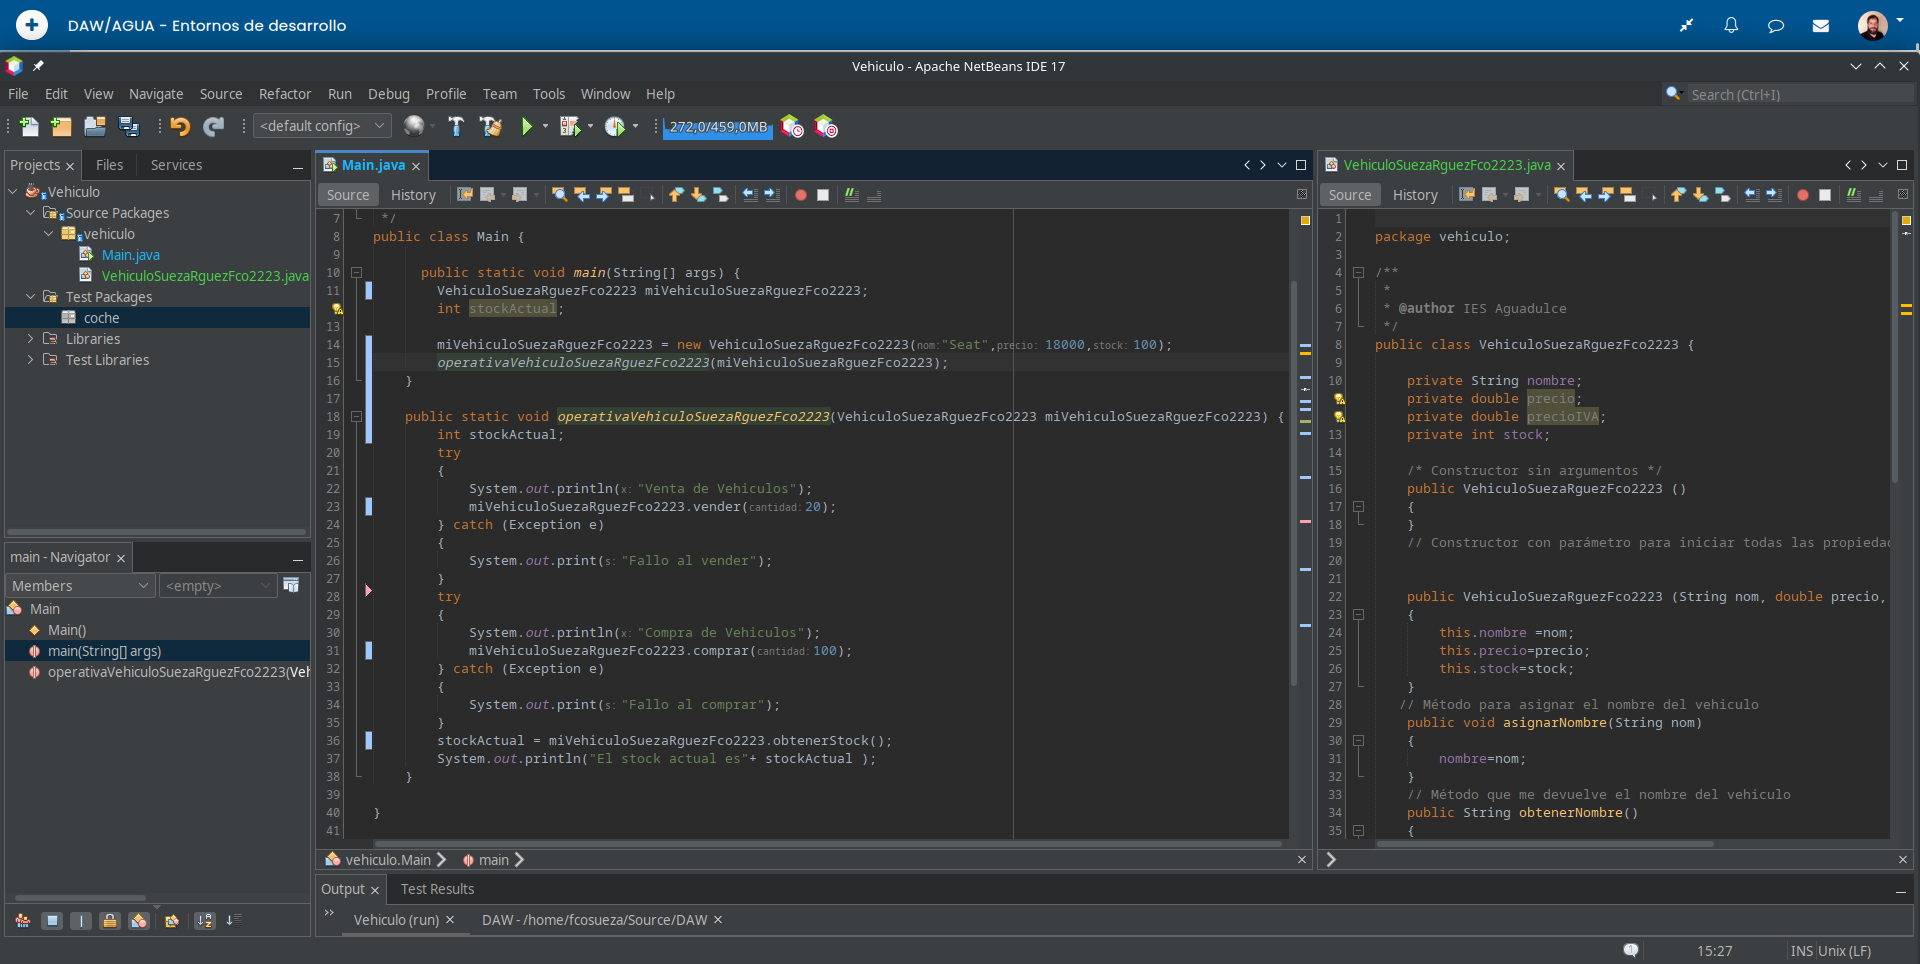
\includegraphics[scale=0.23]{refactor-method-2.png}
        \caption{Clase Main refactorizada con el método añadido y su llamada}
    \end{figure}

    \item A continuación hemos usado la opción de \textit{encapsulate fields} de Netbeans, lo que crea un conjunto de métodos, getters y setters, para para los atributos de la clase en cuestión. En las siguiente capturas se pueden ver los pasos que hemos seguido.

    \begin{figure}[H]
        \centering
        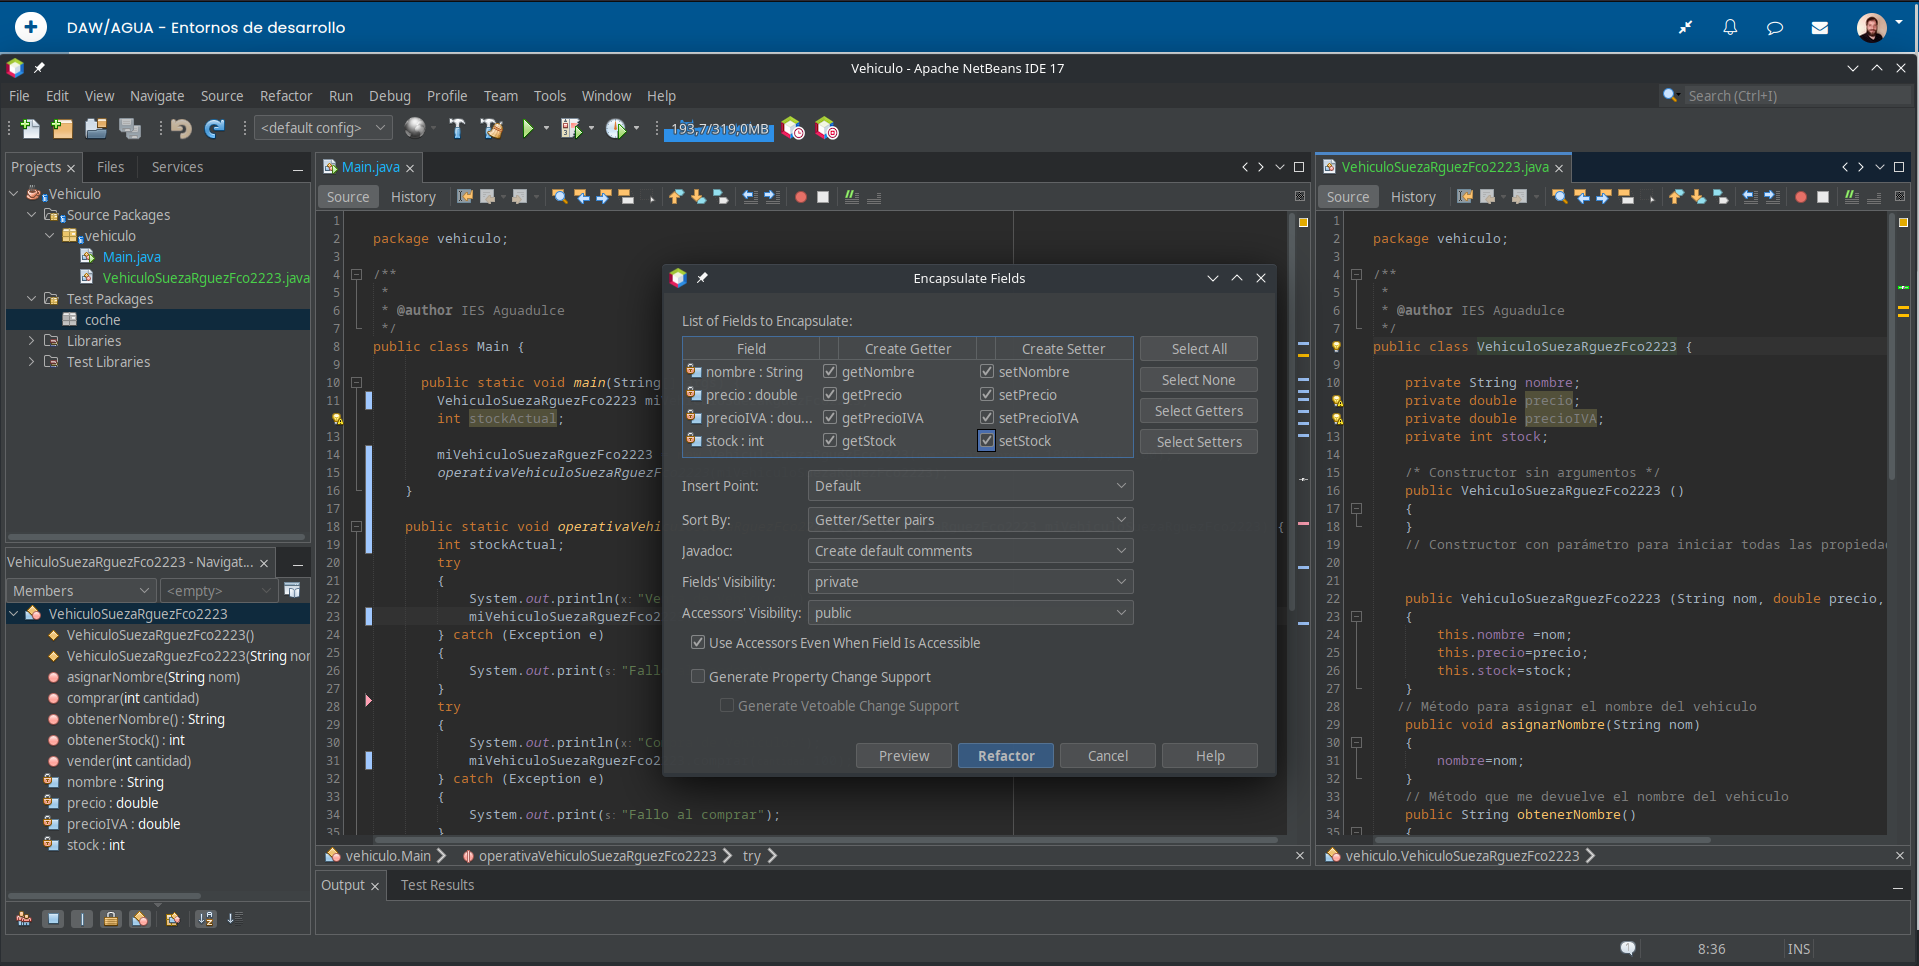
\includegraphics[scale=0.22]{refactor-encap-1.png}
        \caption{Menu encapsulate fields de Netbeans}
    \end{figure}

        \begin{figure}[H]
        \centering
        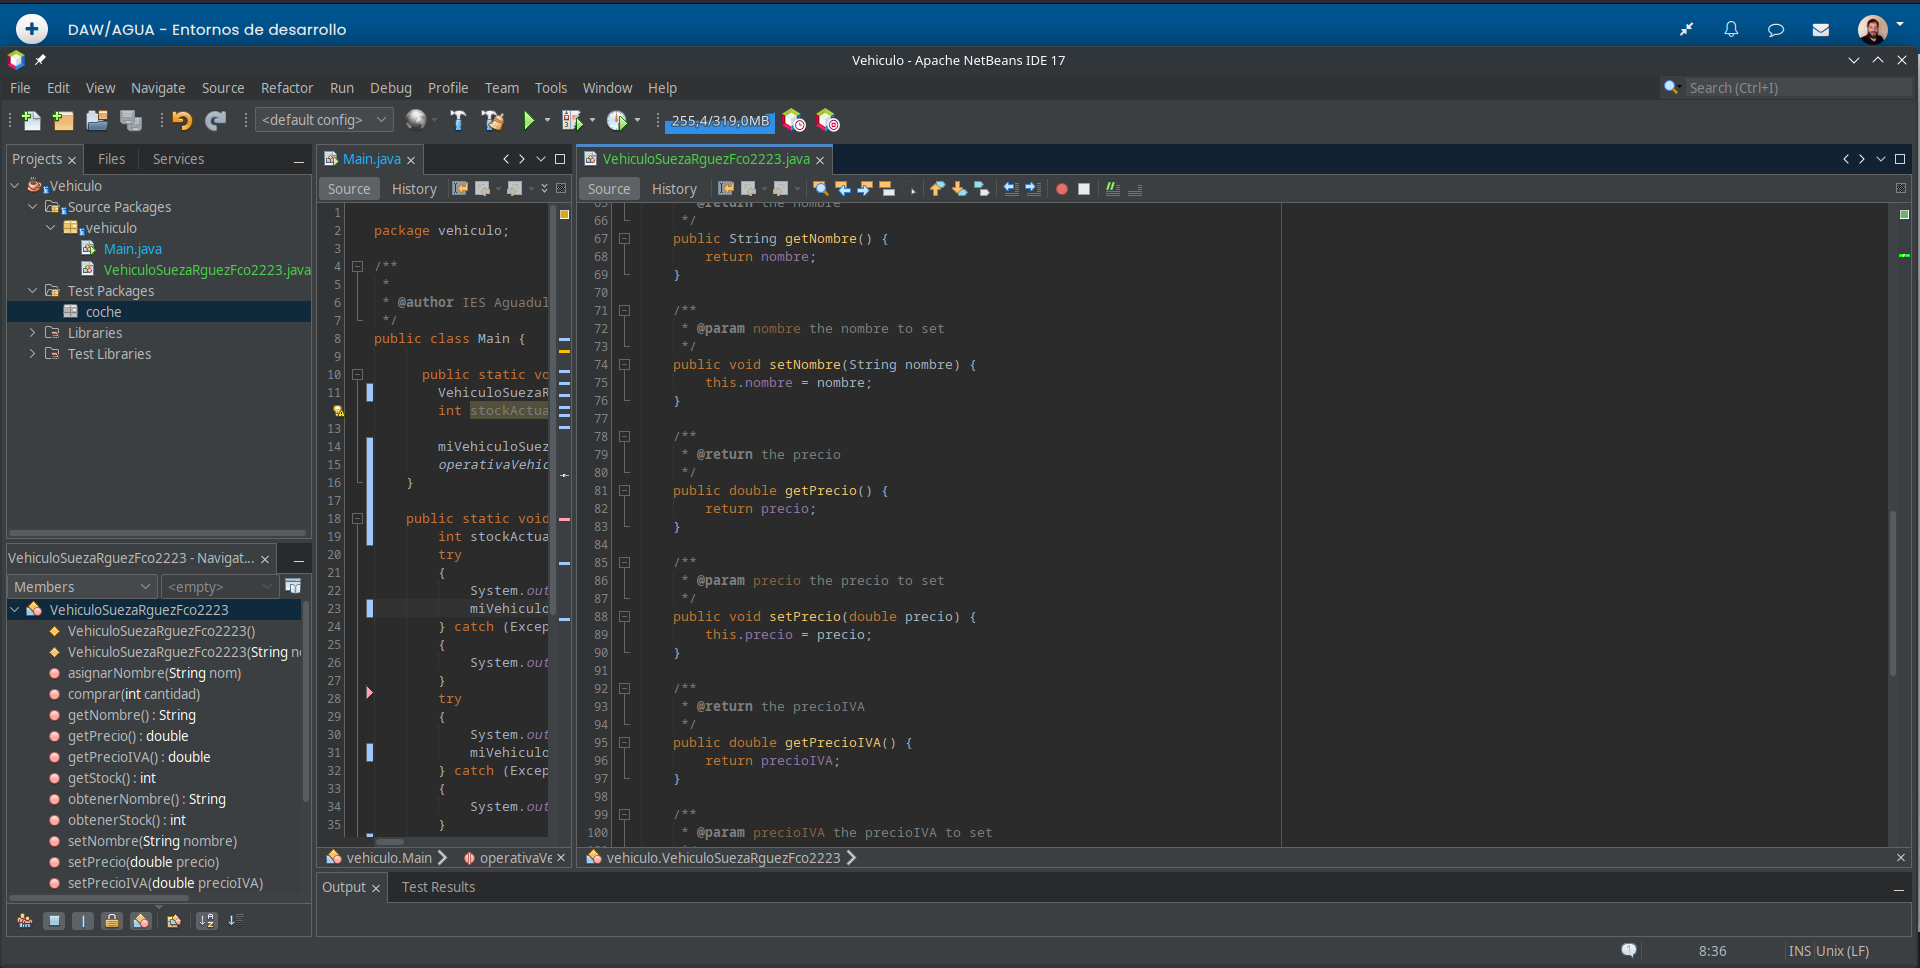
\includegraphics[scale=0.22]{refactor-encap-2.png}
        \caption{Metodos getter y setter agregados}
    \end{figure}

    \item Por último, vamos a añadir una parámetro al método operativaVehiculo. En este caso, será el parámetro \textbf{cantidad} con un \textbf{valor por defecto} de \textbf{50}. Lo hemos realizado usando la opción \textit{Change method parameters} del menú \textit{refactor} de Netbeans, como vemos en las siguiente capturas.

    \begin{figure}[H]
        \centering
        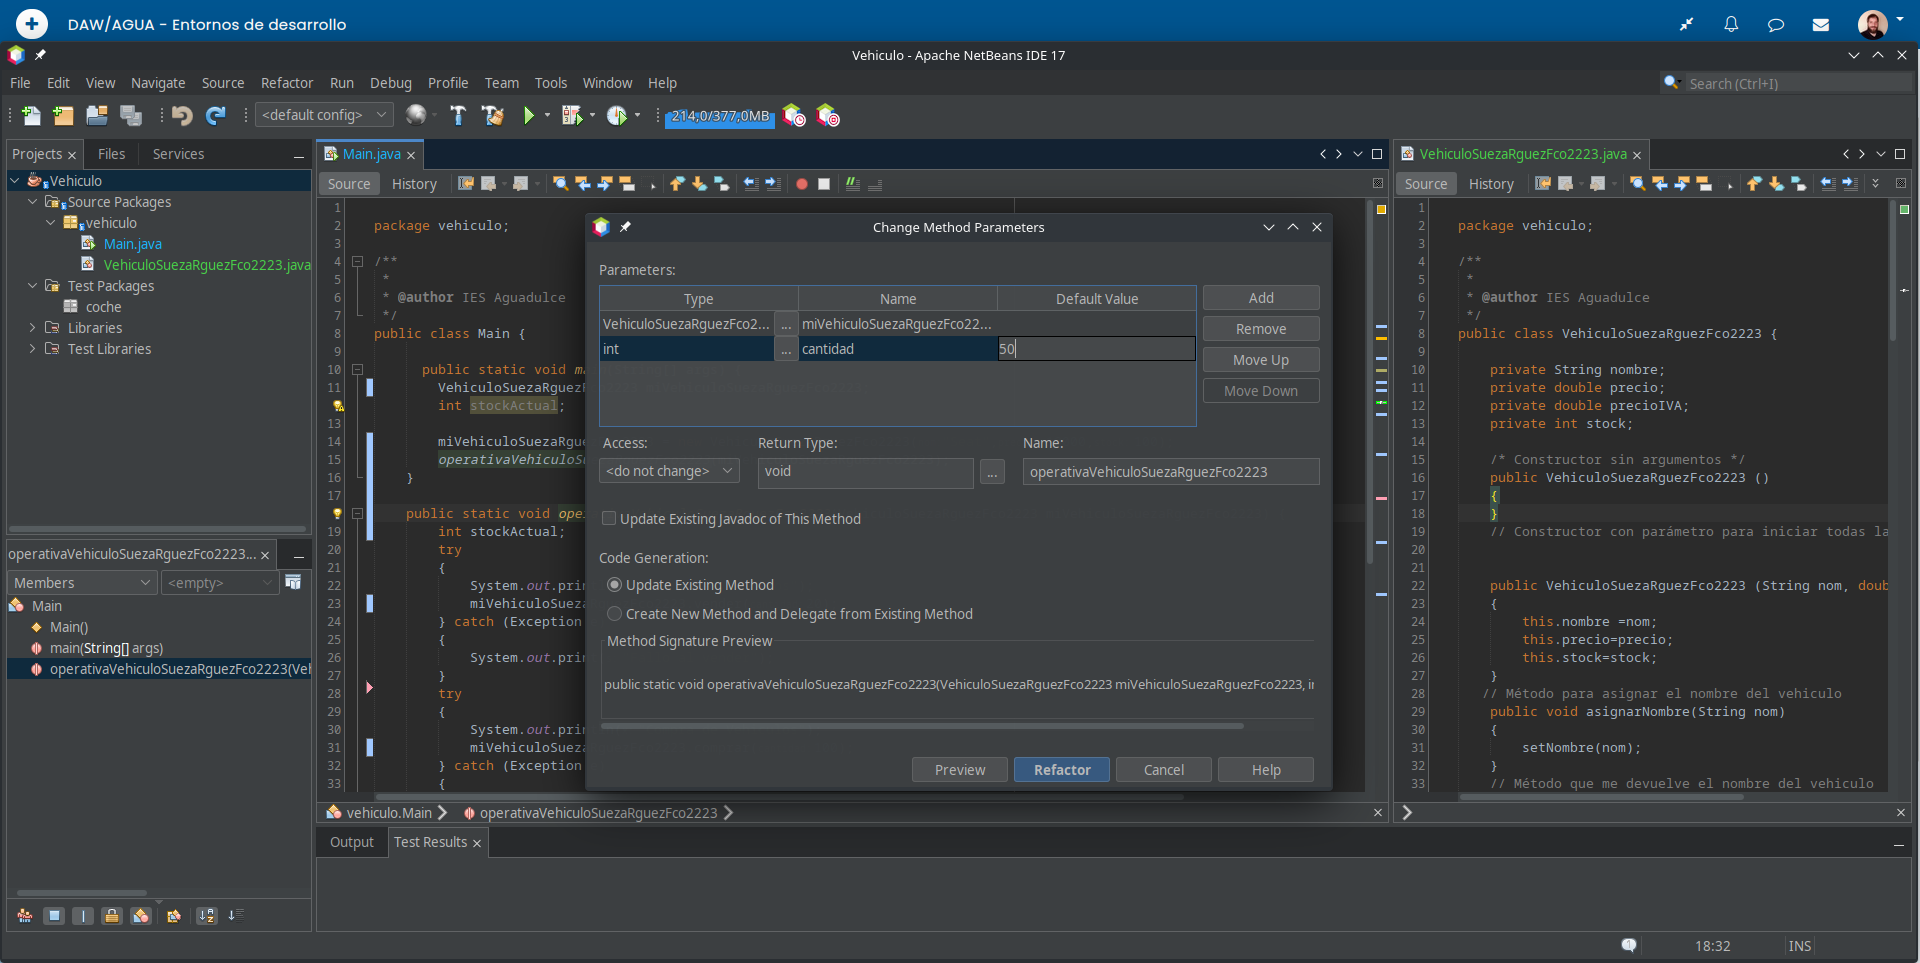
\includegraphics[scale=0.22]{refactor-param.png}
        \caption{Menu Change method parameters de Netbeans}
    \end{figure}

     \begin{figure}[H]
         \centering
        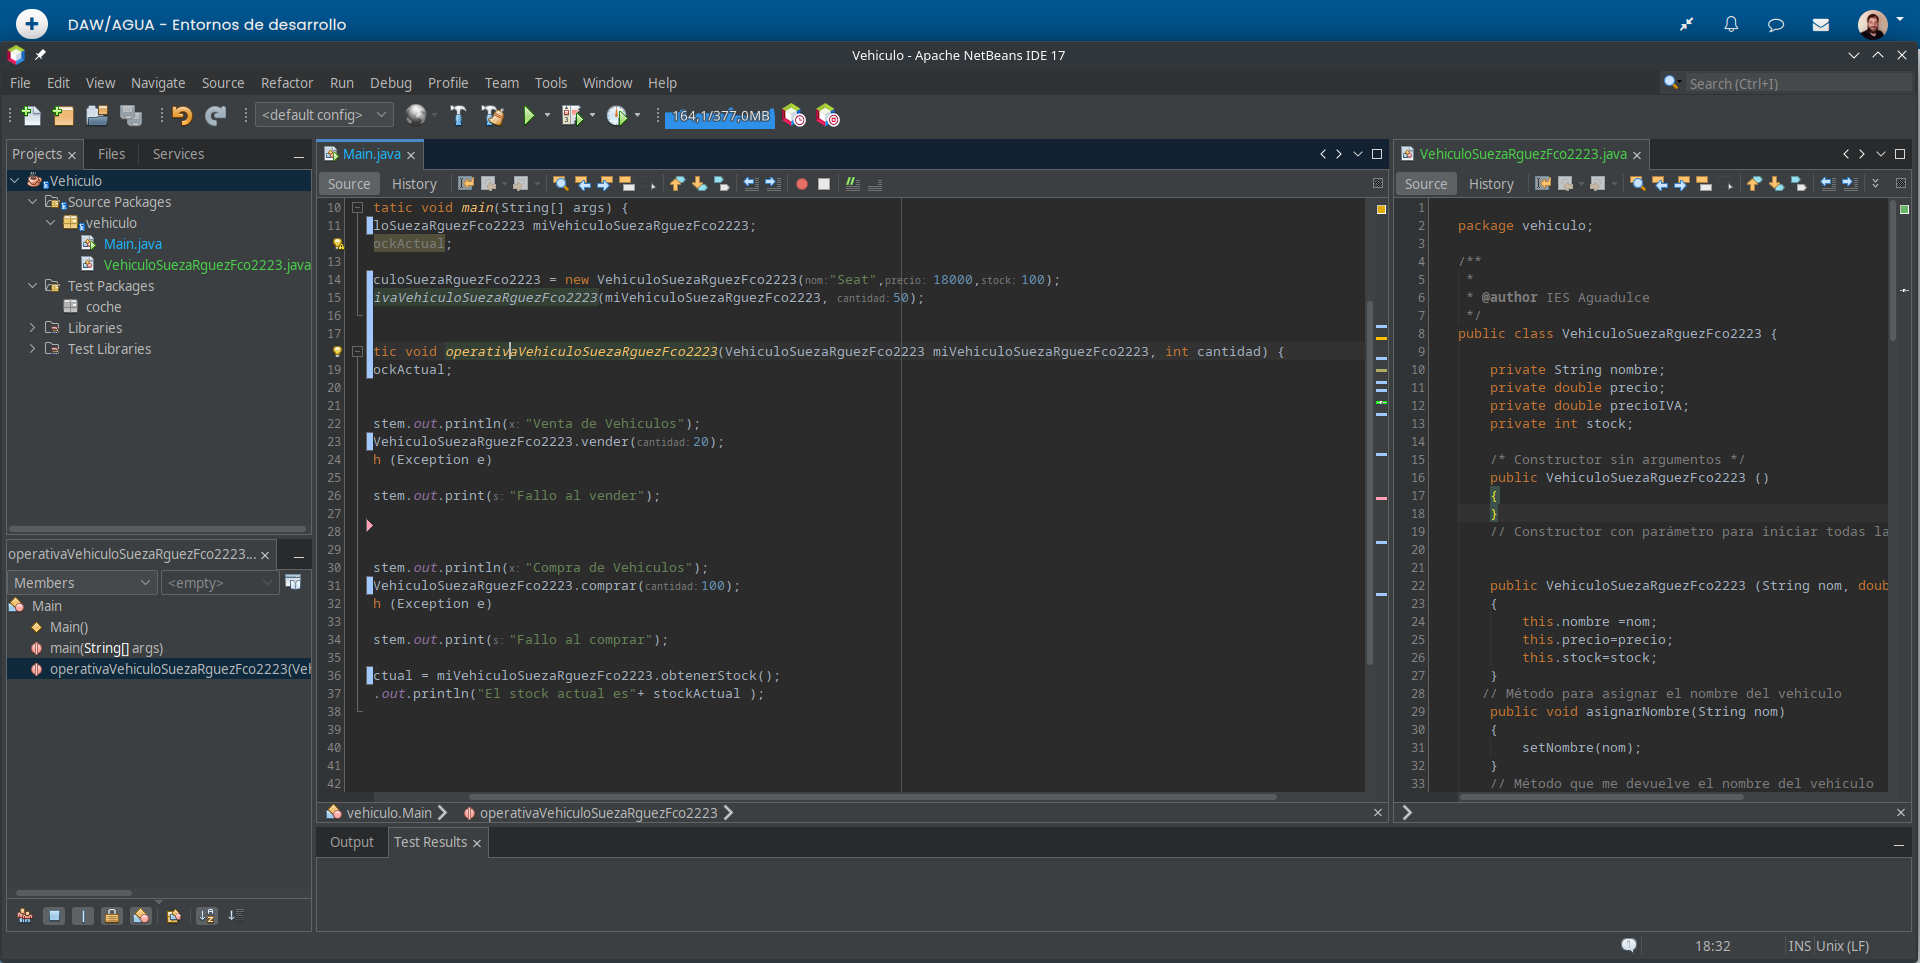
\includegraphics[scale=0.22]{refactor-param-2.png}
        \caption{Método con el nuevo parámetro añadido}
    \end{figure}
\end{enumerate}

\subsection{Actividad 2: Realizar un Análisis de Código}
\subsubsection{Enunciado}
\begin{enumerate}
    \item  Instala el plugin SonarLint en NetBeans (del autor FICHET Philippe). Analiza el código del proyecto con el analizador de código SonarLint. Muestra en una captura los resultados y coméntalos .

    \item Elimina en SonarLint la regla "Unused method parameters should be removed". Analiza de nuevo y, muestra la captura del resultado.
\end{enumerate}

\subsubsection{Solución}
En este apartado vamos a instalar SonarLint, un plugin para Netbeans que realiza análisis estático de código. El proceso de instalación no se va a documentar, ya que se ha tratado en temas anteriores la instalación de plugins, sino que se va a mostrar su ejecución y los resultados, así como comentar los resultados que se han obtenido.

\begin{itemize}
    \item En primer lugar se ha ejecutado SonarLint, lo cual nos ha devuelto varios errores como podemos ver en la siguiente captura.

    \begin{figure}[H]
        \centering
        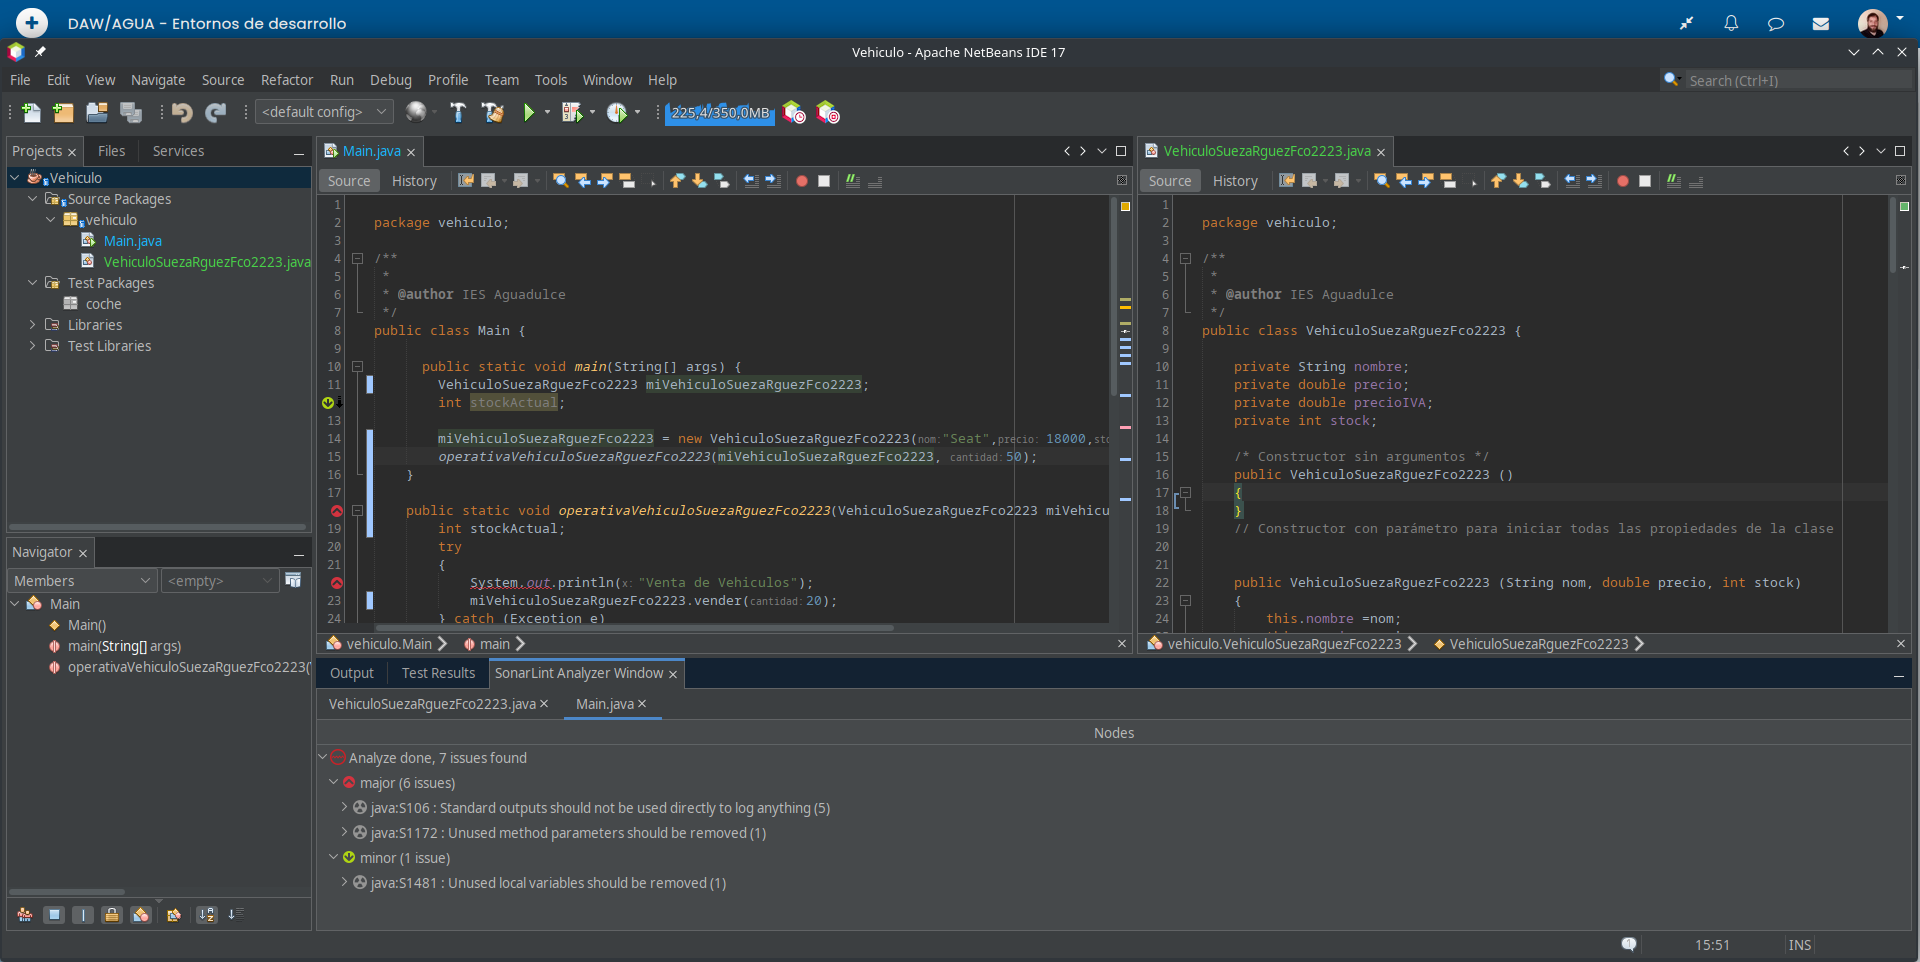
\includegraphics[scale=0.25]{linting.png}
        \caption{Resultado de la ejecución de SonarLint}
    \end{figure}

    \item Ahora pasaremos a comentar los resultados obtenidos:

    Como vemos, el linter nos arroja varios errores. De estos errores 6 son ``graves'' y 1 tiene menos importancia.

    De los 6 errores, 5 nos informan de que no se debe usar la salida estandar (System.out) para loggear nada. Ya que es una mala práctica. El error restante nos informa de que hay un parámetro que no esta siendo usado en un método, en concreto, en la línea 17. Si nos vamos a esa línea vemos que el método operativaVehiculoSuezaRguezFco2223 no esta usando el parámetro cantidad, por lo que solo habría que eliminar ese parámetro, pero nosotros vamos a eliminar la regla que hace que nos suelte ese error, como vemos en el punto siguiente.

    \item En este punto, como hemos comentado, vamos a modificar la regla "Unused method parameters should be removed", para que deje de mostrarnos el error que hemos comentado en el punto anterior. En nuestro caso, si pulsamos en la opción del menú \textit{Windows}, la primera opción que nos aparece es \textit{Sonar Rules Detail}.

    Al pulsar se nos abrirá una ventada abajo, mostrando todas las reglas configuradas para SonarLint. Algunas no viene con el nombre, sino con un código tipo \textit{java:S1172}, como es nuestro caso, en el que la regla que queremos deshabilitar tiene precisamente ese nombre, \textbf{java:S1172}.

    \begin{figure}[H]
        \centering
        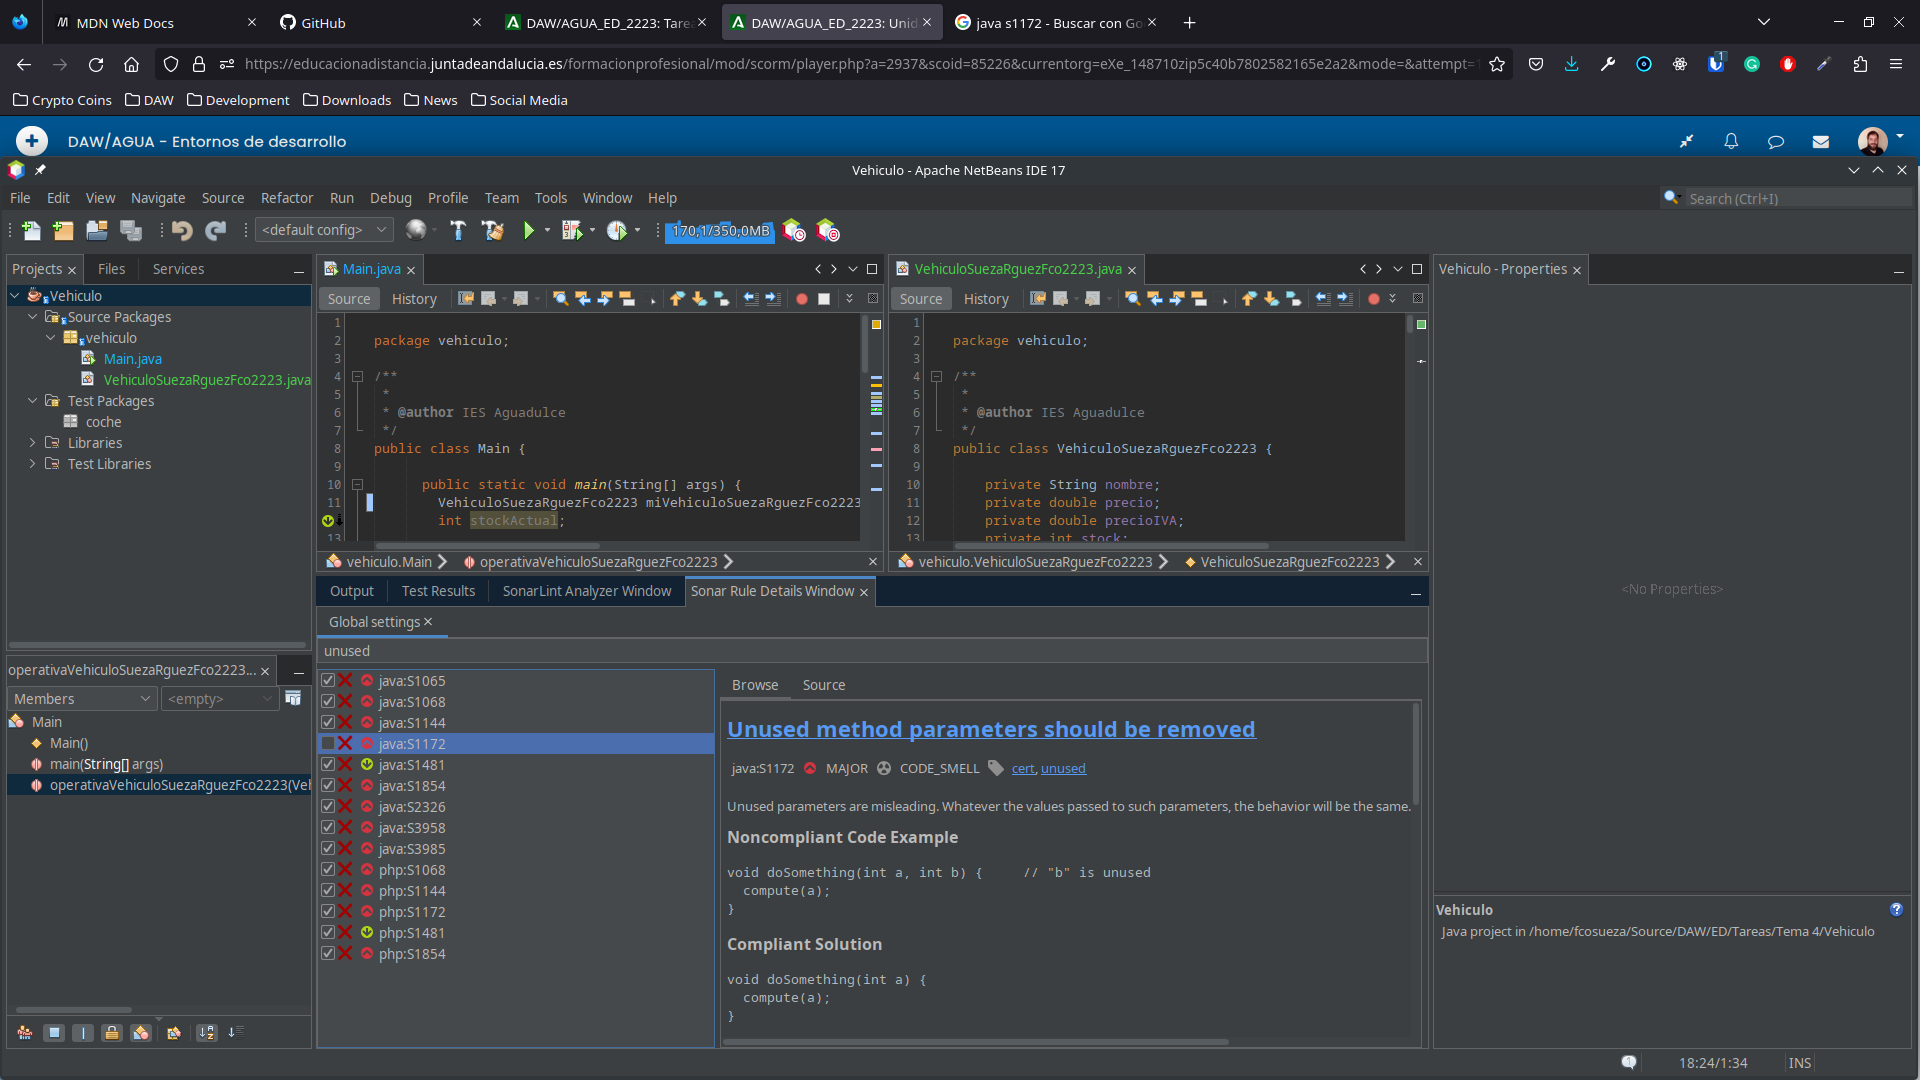
\includegraphics[scale=0.22]{linting-rule-1.png}
        \caption{Desactivación de la regla Unused method parameters should be removed}
    \end{figure}

    Si desactivamos la opción y volvemos a pasar el linter, veremos que ya no nos muestra el error relativo al parámetro sin usar en el método operativaVehiculoSuezaRguezFco2223, como podemos ver en la siguiente captura.

        \begin{figure}[H]
        \centering
        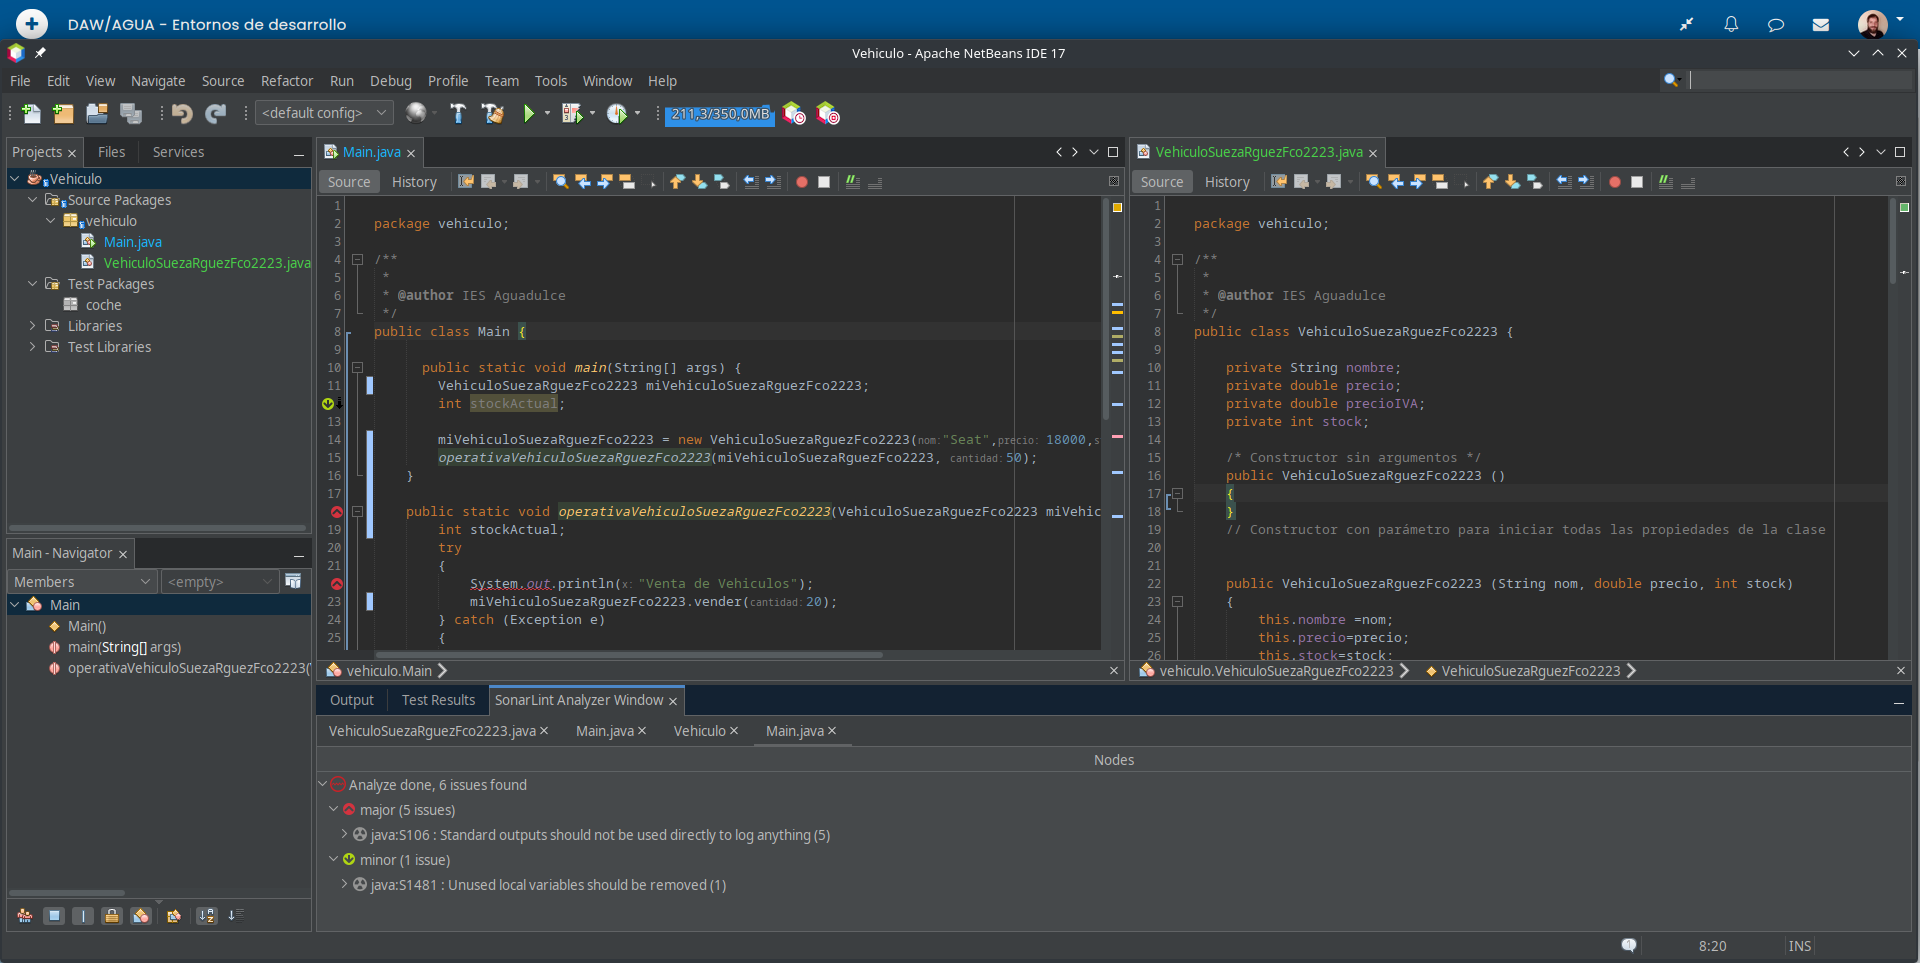
\includegraphics[scale=0.22]{linting-rule-2.png}
        \caption{Resultado de SonarLint despues de desactivar la opción}
    \end{figure}
\end{itemize}

\subsection{Actividad 3: Control de Versiones con Github}
\subsubsection{Enunciado}
\begin{enumerate}
    \item Entra en GitHub (si no tienes cuenta la tienes que crear) y crea un repositorio con el nombre VehiculoXXX2223 (donde XXX son tus iniciales).

    \item Inicializa el control de versiones con Git en tu proyecto local de Netbeans y haz un commit con el comentario "Mi primer commit XXX2223".

    \item Realiza un push del proyecto VehiculoXXX2223, muestra el contenido del proyecto en tu cuenta de GitHub y copia en el documento el enlace a su repositorio.
\end{enumerate}

\subsubsection{Solución}
En este aparatado vamos a usar el sistema de control de versiones Git y en concreto su interfaz web Github. En mi caso, ya tengo una cuenta de Github, por lo que no ha sido necesario crearme una.

\begin{enumerate}
    \item En primer lugar, hemos creado un repositorio en Github con el nombre VehiculoFJS2223. como vemos en la siguiente captura.

    \begin{figure}[H]
        \centering
        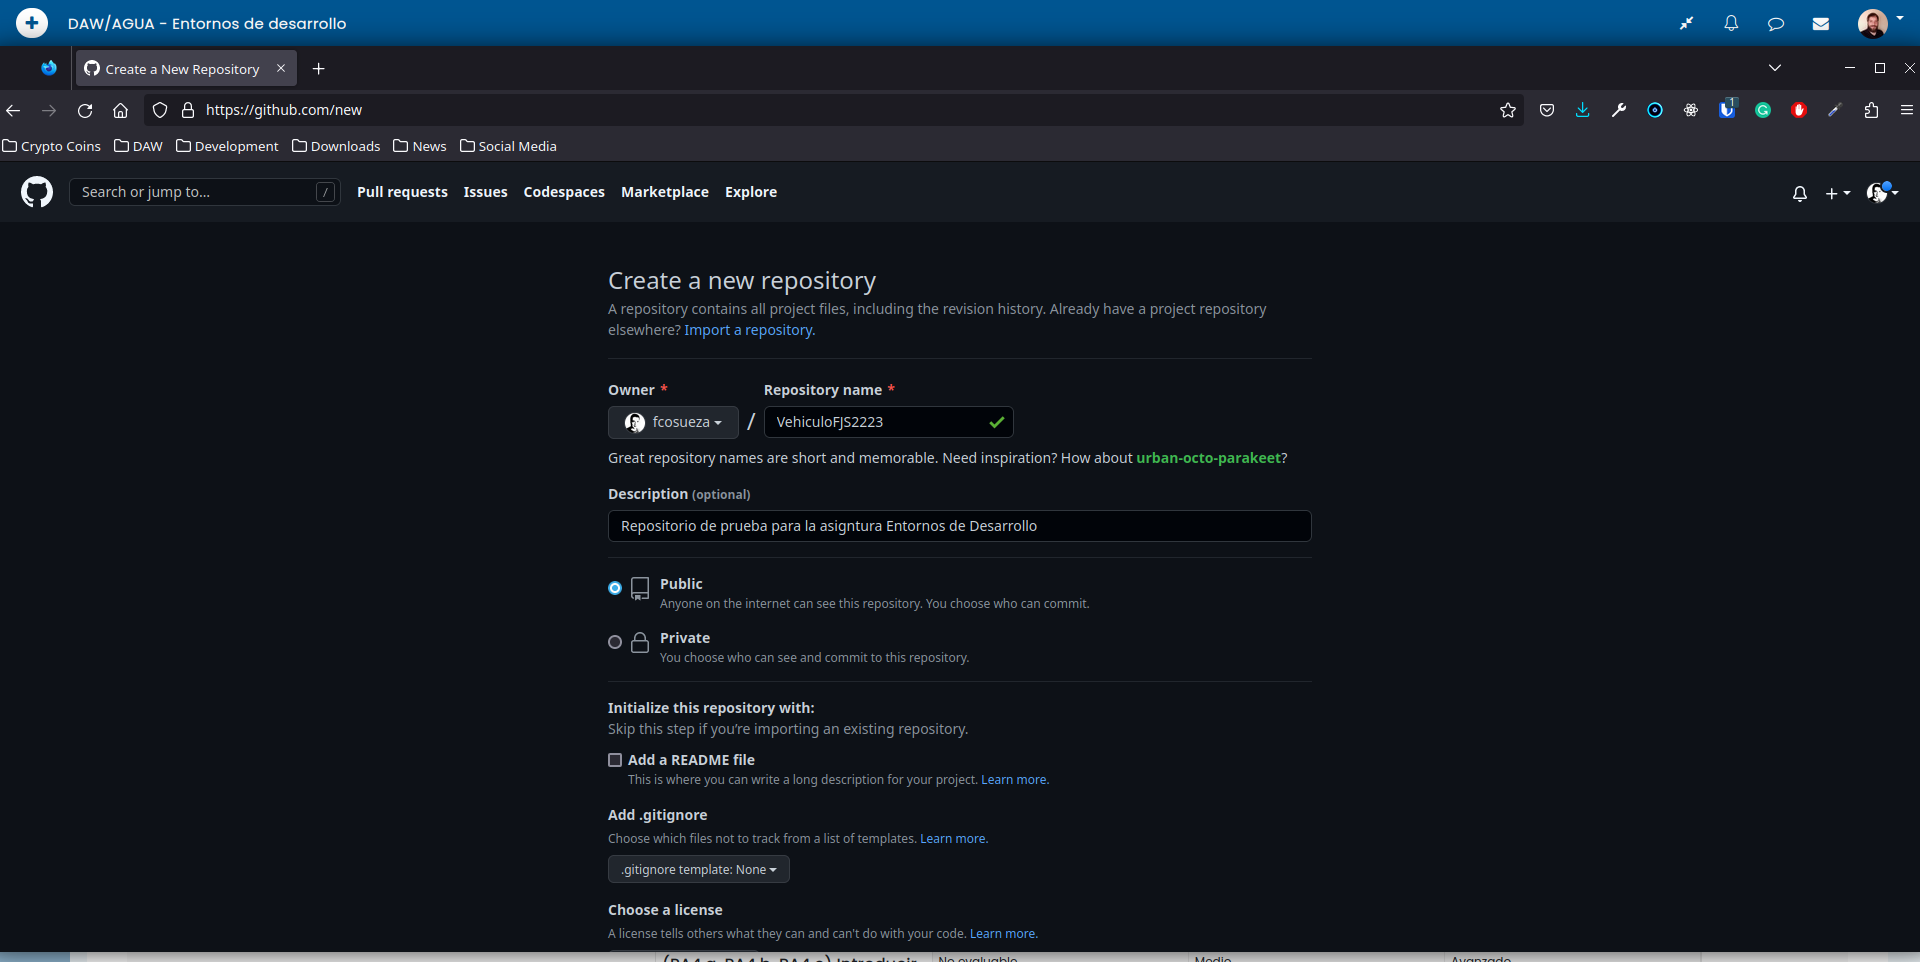
\includegraphics[scale=0.25]{github-create.png}
        \caption{Creación del repositorio en Github}
    \end{figure}

    \item A continuación, hemos inicializado un repositorio Git con Netbeans para nuestro proyecto y hemos realizado un primer commit.

    \begin{figure}[H]
        \centering
        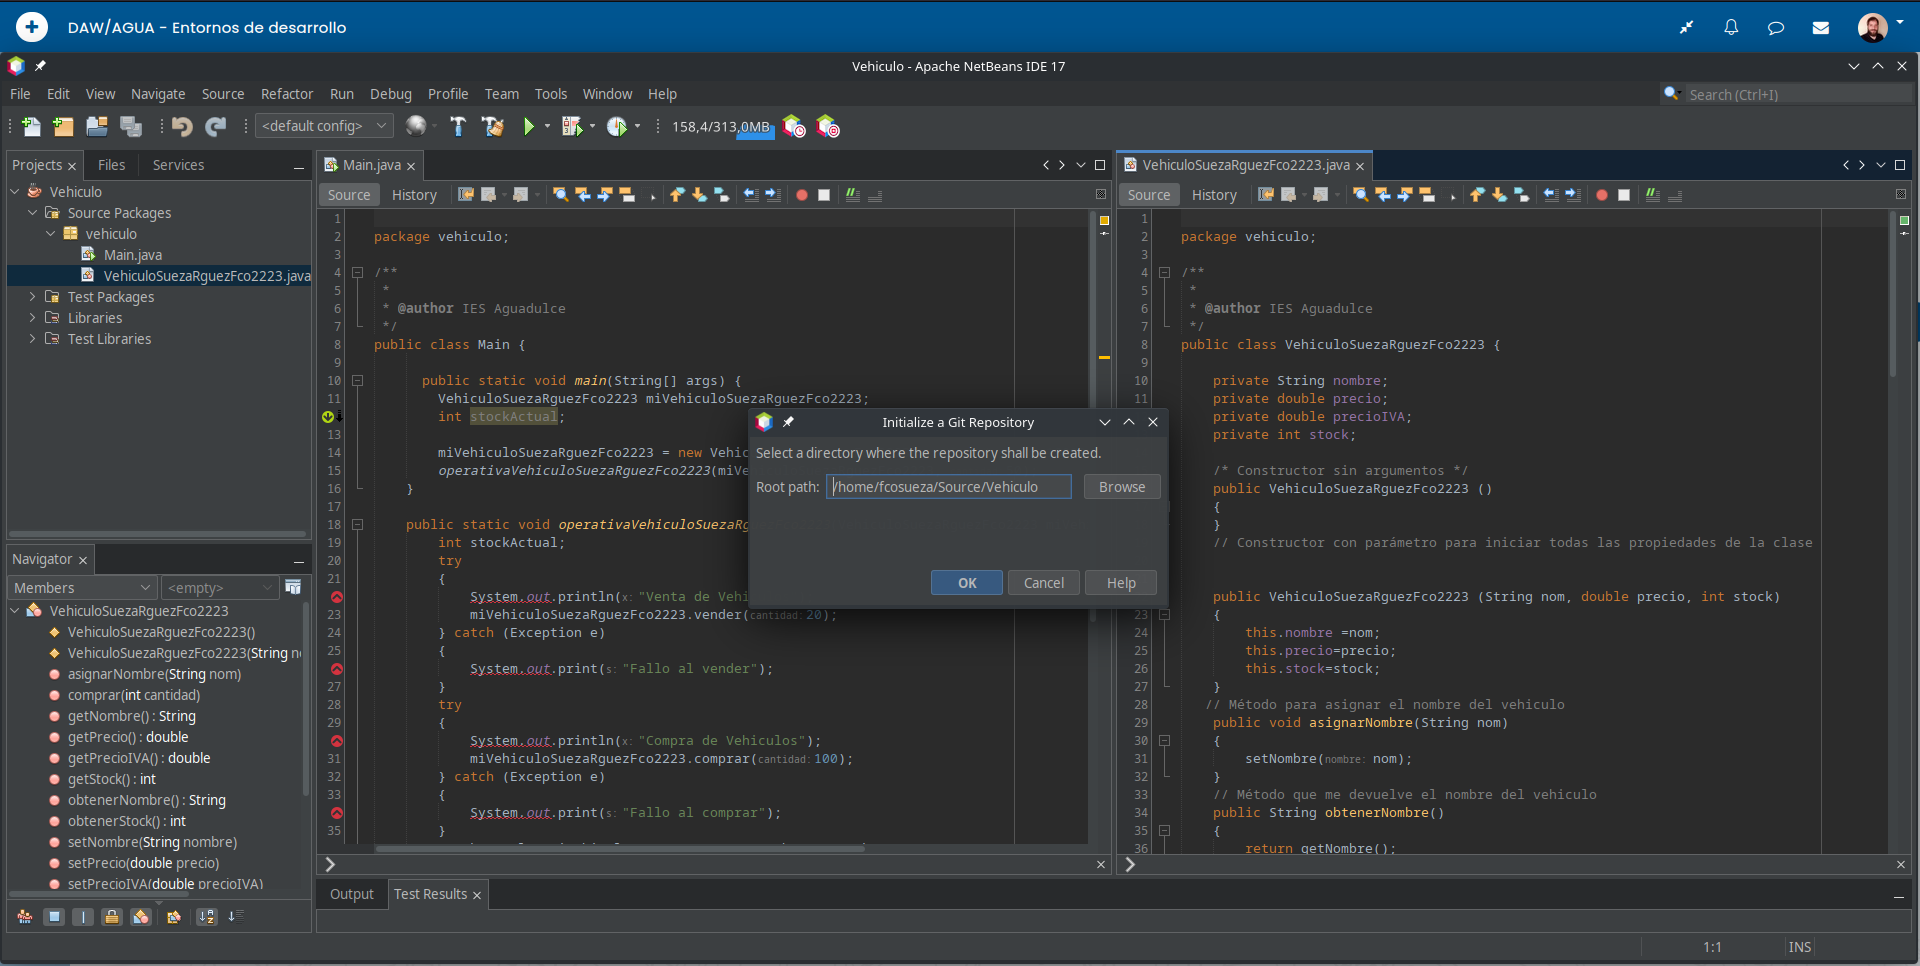
\includegraphics[scale=0.25]{github-netbeans.png}
        \caption{Inicialización de proyecto Git con Netbeans}
    \end{figure}


    \begin{figure}[H]
        \centering
        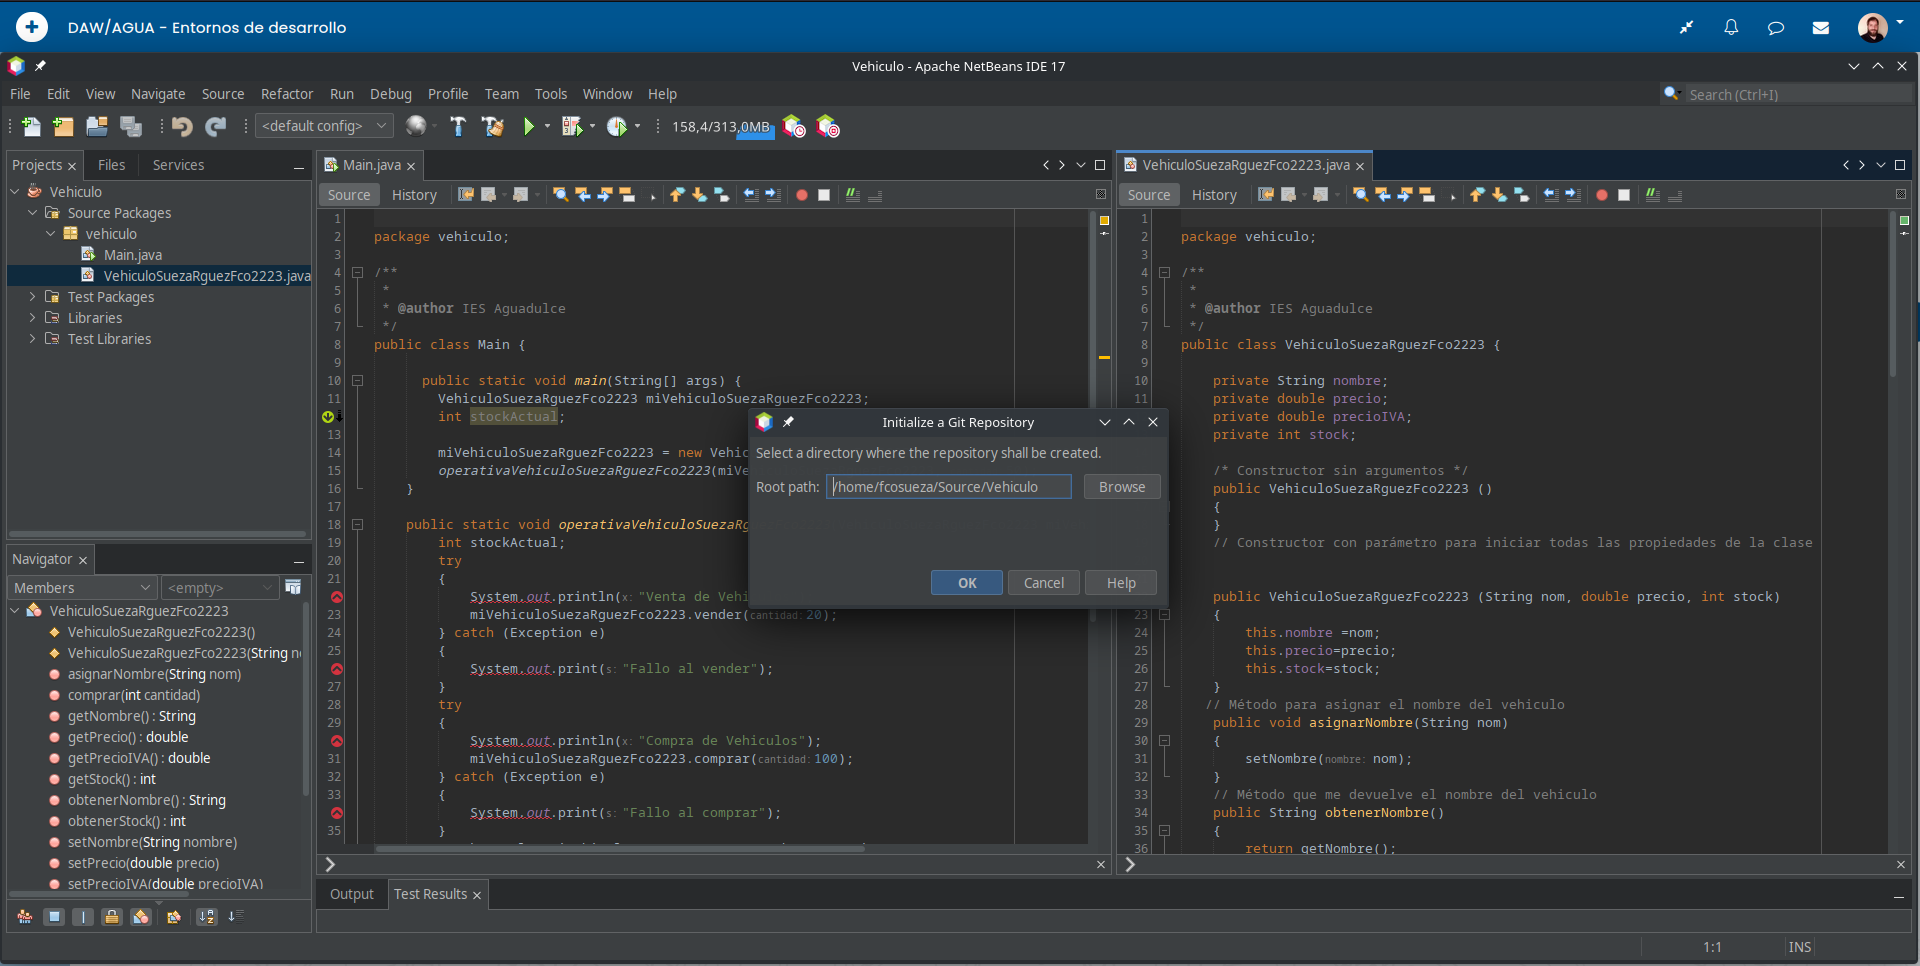
\includegraphics[scale=0.25]{github-netbeans.png}
        \caption{Primer commit de nuestro repositorio}
    \end{figure}

        \item Por ultimo, vamos a realizar un \textbf{push} a nuestro\textbf{ repositorio remoto}. Para ello habrá que especificar nuestro repositorio remoto en el menú que nos mostrará Netbeans, donde se nos pedirá información sobre la url del proyecto, nuestro usuario, como nos vamos a autentificar, en nuestra caso es usando la \textbf{clave publica SSH}, aunque también se puede hacer mediante un token HTML o incluyendo el usuario y la contraseña de Github. En la siguiente captura, podemos ver como ha quedado el repositorio después de realizar push.

     \begin{figure}[ht]
        \centering
        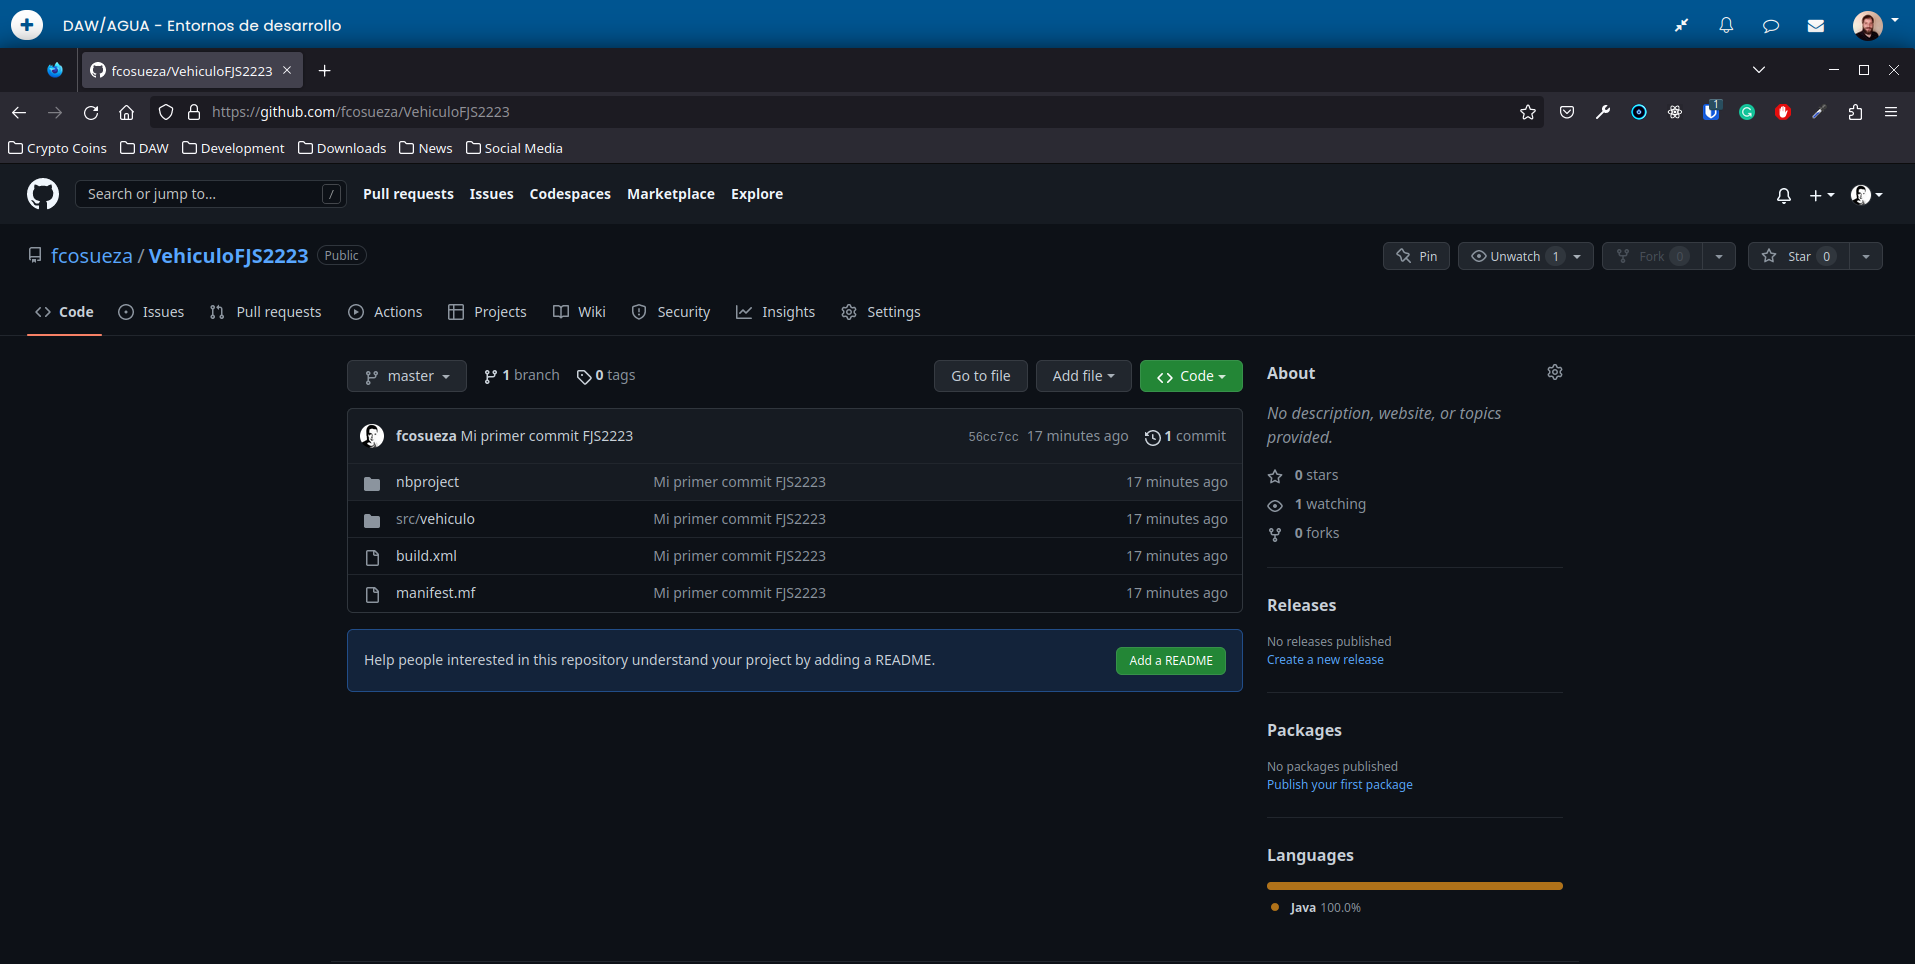
\includegraphics[scale=0.25]{github-repo.png}
        \caption{Repositorio de Github tras pushear el primer commit}
    \end{figure}

    Una vez realizado el commit, ya aparecerá en el historial, indicando cuando se realizó y que cambios se incluyeron en el repositorio.

    Además de este commit, hemos añadido un más creando un README para explicar un poco el propósito del repositorio.
    En la url, podemos visitar este repositorio:

    \begin{itemize}
        \item \url{https://github.com/fcosueza/VehiculoFJS2223}
    \end{itemize}
\end{enumerate}

\subsection{Actividad 4: Documentación del Código}
\subsubsection{Enunciado}
\begin{enumerate}
    \item Comenta cada uno de los elementos principales de la clase VehiculoXXX2223 y de la clase Main siguiendo las normas de javadoc.
    \item Genera documentación Javadoc para todo el proyecto.
\end{enumerate}

\subsubsection{Solución}
\begin{enumerate}
    \item En primer lugar se ha procedido a comentar, usando la sintaxis de Javadoc, todos los métodos y las clases del proyecto.

    \begin{figure}[ht]
        \centering
        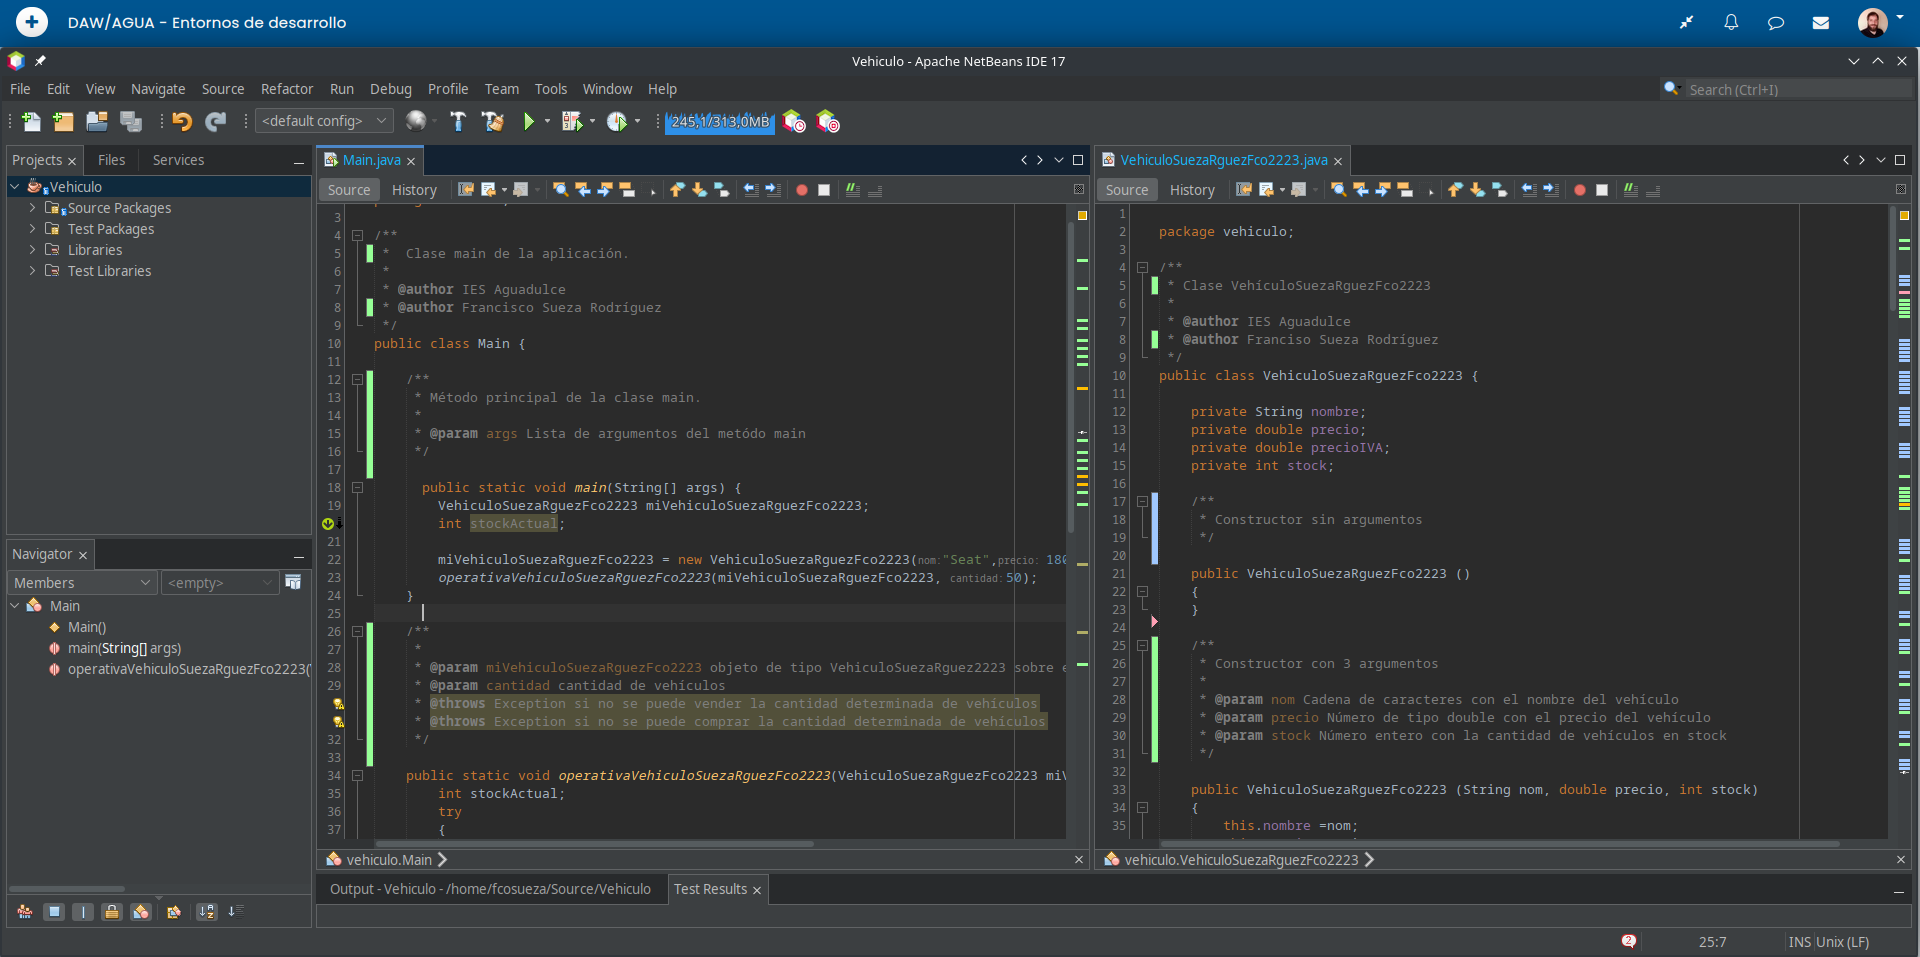
\includegraphics[scale=0.23]{javadoc.png}
        \caption{Documentación de clases y métodos}
    \end{figure}

    \item A continuación, se ha generado la documentación.

    \begin{figure}[ht]
        \centering
        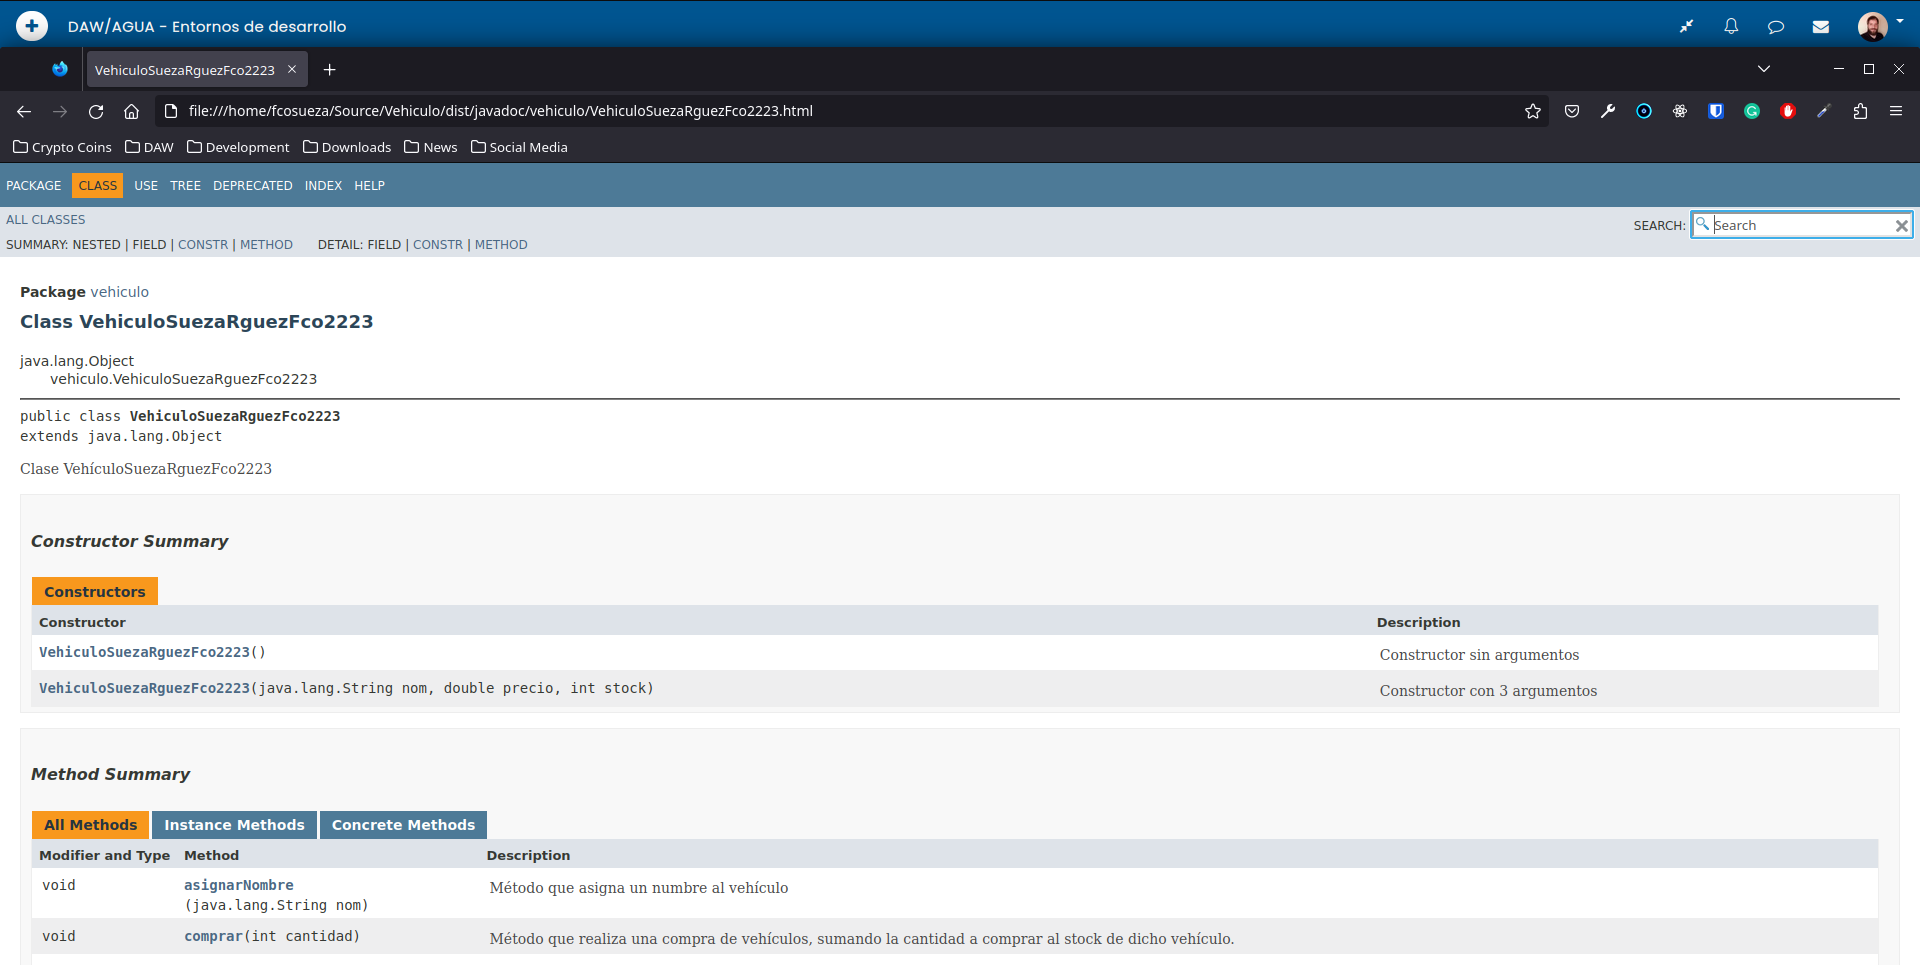
\includegraphics[scale=0.23]{javadoc-2.png}
        \caption{Página de la documentación generada}
    \end{figure}
\end{enumerate}

Por último, destacar que se ha realizado un commit y push de los cambios realizados en el proyecto, por lo que aparecerán reflejados en el repositorio de éste.


% Bibliography
%\newpage
%\bibliography{citas}
%\bibliographystyle{unsrt}

\end{document}